\documentclass[letterpaper]{article} % DO NOT CHANGE THIS
\usepackage[submission]{aaai2027}  % DO NOT CHANGE THIS
% The serif, sans-serif, and monospaced fonts are loaded automatically by
% aaai2027.sty (newtxtext, helvet, courier). DO NOT add \usepackage{times},
% \usepackage{helvet}, \usepackage{courier}, or any other font package.
\usepackage[hyphens]{url}  % DO NOT CHANGE THIS
\usepackage{graphicx} % DO NOT CHANGE THIS
\urlstyle{rm} % DO NOT CHANGE THIS
\def\UrlFont{\rm}  % DO NOT CHANGE THIS
\usepackage{natbib}  % DO NOT CHANGE THIS AND DO NOT ADD ANY OPTIONS TO IT
\usepackage{caption} % DO NOT CHANGE THIS AND DO NOT ADD ANY OPTIONS TO IT
\frenchspacing  % DO NOT CHANGE THIS
%
% These are recommended to typeset algorithms but not required. See the subsubsection on algorithms. Remove them if you don't have algorithms in your paper.
\usepackage{algorithm}
\usepackage{algorithmicx}
\usepackage{algcompatible}
\usepackage{algpseudocode}

\usepackage{multirow}
\usepackage{makecell}

\usepackage{amsmath}
\usepackage{amssymb}

%
% These are recommended to typeset listings but not required. See the subsubsection on listing. Remove this block if you don't have listings in your paper.
\usepackage{newfloat}
\usepackage{listings}
\DeclareCaptionStyle{ruled}{labelfont=normalfont,labelsep=colon,strut=off} % DO NOT CHANGE THIS
\lstset{%
	basicstyle={\footnotesize\ttfamily},% footnotesize acceptable for monospace
	numbers=left,numberstyle=\footnotesize,xleftmargin=2em,% show line numbers, remove this entire line if you don't want the numbers.
	aboveskip=0pt,belowskip=0pt,%
	showstringspaces=false,tabsize=2,breaklines=true}
\floatstyle{ruled}
\newfloat{listing}{tb}{lst}{}
\floatname{listing}{Listing}

%
% Recommended for better-looking tables
\usepackage{booktabs}

%
% Keep the \pdfinfo as shown here. There's no need
% for you to add the /Title and /Author tags.
\pdfinfo{
/TemplateVersion (2027.1)
}

\usepackage{caption}
\usepackage{algorithm}
\usepackage{algpseudocode}
\usepackage{amsthm}
\usepackage{amsmath}
\newtheorem{theorem}{Theorem}
\newtheorem{proposition}{Proposition}
\usepackage[colorinlistoftodos]{todonotes}


% DISALLOWED PACKAGES
% \usepackage{authblk} -- This package is specifically forbidden
% \usepackage{balance} -- This package is specifically forbidden
% \usepackage{CJK} -- This package is specifically forbidden
% \usepackage{float} -- This package is specifically forbidden
% \usepackage{flushend} -- This package is specifically forbidden
% \usepackage{fullpage} -- This package is specifically forbidden
% \usepackage{geometry} -- This package is specifically forbidden
% \usepackage{hyperref} -- This package is specifically forbidden
% \usepackage{navigator} -- This package is specifically forbidden
% (or any other package that embeds links such as navigator or hyperref)
% \usepackage{indentfirst} -- This package is specifically forbidden
% \usepackage{layout} -- This package is specifically forbidden
% \usepackage{multicol} -- This package is specifically forbidden
% \usepackage{nameref} -- This package is specifically forbidden
% \usepackage{savetrees} -- This package is specifically forbidden
% \usepackage{setspace} -- This package is specifically forbidden
% \usepackage{stfloats} -- This package is specifically forbidden
% \usepackage{tabu} -- This package is specifically forbidden
% \usepackage{titlesec} -- This package is specifically forbidden
% \usepackage{tocbibind} -- This package is specifically forbidden
% \usepackage{ulem} -- This package is specifically forbidden
% \usepackage{wrapfig} -- This package is specifically forbidden
% DISALLOWED COMMANDS
% \nocopyright -- Your paper will not be published if you use this command
% \addtolength -- This command may not be used
% \balance -- This command may not be used
% \baselinestretch -- Your paper will not be published if you use this command
% \clearpage -- No page breaks of any kind may be used for the final version of your paper
% \columnsep -- This command may not be used
% \newpage -- No page breaks of any kind may be used for the final version of your paper
% \pagebreak -- No page breaks of any kind may be used for the final version of your paper
% \pagestyle -- This command may not be used
% \tiny -- This is not an acceptable font size.
% \vspace{- -- No negative value may be used in proximity of a caption, figure, table, section, subsection, subsubsection, or reference
% \vskip{- -- No negative value may be used to alter spacing above or below a caption, figure, table, section, subsection, subsubsection, or reference

\setcounter{secnumdepth}{0} %May be changed to 1 or 2 if section numbers are desired.

% The file aaai2027.sty is the style file for AAAI Press
% proceedings, working notes, and technical reports.
%

% Title

% Your title must be in mixed case, not sentence case.
% That means all verbs (including short verbs like be, is, using,and go),
% nouns, adverbs, adjectives should be capitalized, including both words in hyphenated terms, while
% articles, conjunctions, and prepositions are lower case unless they
% directly follow a colon or long dash
\title{CAST: Constrained Assignment of Symbolic Types \\ for Online Model Repair in Planning }
\author{Anonymous Submission}
\affiliations{}
% \usepackage[disable,colorinlistoftodos]{todonotes} % uncomment for diabling
\newcommand{\BMK}[1]{\todo[inline,color=cyan!25]{BMK: #1}}
\newcommand{\SG}[1]{\todo[inline,color=yellow!25]{SG: #1}}
\newcommand{\JS}[1]{\todo[inline,color=red!25]{JS: #1}}

% ============================================================
% CAST pipeline figure (Fig. 1) -- native TikZ rendering
% ============================================================
\usepackage{tikz}
\usetikzlibrary{positioning,arrows.meta,fit,backgrounds,calc}

% palette
\definecolor{pkw}{RGB}{28,90,168}      % define / domain / problem
\definecolor{psec}{RGB}{140,55,150}    % :types :objects :init :goal ...
\definecolor{ptype}{RGB}{18,132,80}    % LLM-assigned functional types
\definecolor{panelbg}{RGB}{248,249,251}
\definecolor{panelrule}{RGB}{205,210,218}
\definecolor{hdrbg}{RGB}{233,238,245}
\definecolor{stagebg}{RGB}{252,252,253}
\definecolor{stagerule}{RGB}{120,128,140}
\definecolor{accent}{RGB}{40,70,120}

% PDDL as a listings language
\lstdefinelanguage{PDDL}{
  alsoletter={:-_},
  morekeywords={define,domain,problem},
  morekeywords=[2]{:requirements,:strips,:typing,:types,:objects,:init,:goal,:domain},
  sensitive=true,
}
\lstdefinestyle{pddl}{
  language=PDDL,
  basicstyle=\footnotesize\ttfamily,
  keywordstyle=\color{pkw}\bfseries,
  keywordstyle=[2]\color{psec}\bfseries,
  numbers=none,
  showstringspaces=false,
  columns=fullflexible,
  keepspaces=true,
  aboveskip=0pt,belowskip=0pt,xleftmargin=2pt,
}
% typed-problem variant: highlight the functional types the LLM assigns
\lstdefinestyle{pddltyped}{style=pddl,
  emph={robot,graspable,blackboard},
  emphstyle={\color{ptype}\bfseries},
}

\newsavebox\pddlDomA
\newsavebox\pddlProbU
\newsavebox\pddlDomB
\newsavebox\pddlProbT
\newlength\panelw   % common width for all code panels (set in the figure)

% a titled code panel: #1 = header text, #2 = saved code box
\newcommand{\pddlpanel}[2]{%
  \begin{tikzpicture}[inner sep=0pt]
    \node[fill=hdrbg,rounded corners=2pt,inner xsep=6pt,inner ysep=2pt,
          font=\scriptsize\bfseries,text=accent] (h) {#1};
    \node[below=1.2pt of h.south west,anchor=north west,
          fill=panelbg,draw=panelrule,rounded corners=2pt,inner sep=4pt]
          {\makebox[\panelw][l]{#2}};
  \end{tikzpicture}%
}

\begin{document}

\maketitle

% - PDDL problems can have mistakes in them. Plan repair literature for example looks at invalid PDDL and attempts to repair it (symbolically). Maybe human error introduced a typing gap or perhaps we were generating the problem at run time from an open vocabulary system like DINO, the reason does not really matter, there are different ways to end up with a typing gap.

% - Domain files for open world PDDL can be thought of in a way as something provided from the factory --- all of the actions that robot is capable of and the type of objects these actions can be applied to can be enumerated (of course this would be hard to enumerate, thus why we are talking about composition). This means we assume these actions and types are given to us.

% - Our job is to close the gap, we have a problem that is not solvable due to a typing gap so we ask an LLM to retype objects such that the typing gap is closed.

% - It is important to consider cases where the typing gap cannot be closed - no valid substitute is available. We want to fail gracefully.

% - Typing needs to be done with respect to the goal --- for example an object being blue is irrelevant if we are concerned with a different property such as friction. Thus this is hard to do symbolically, but as humans we are good at it.

% - Our example problems have hand annotated ground truth files --- that is we enumerate valid substitutions to ensure that the LLM is not assigning a brick to be used in place of a cloth. 

% - APB (and solutions that have the LLM generate a final plan in general) are not exactly a direct comparison to this approach. Because they use LLMs and are thus less rigid, they just happen to be willing willing to solve typing gaps. 



% 
\begin{abstract} 

Symbolic planners provide systematic search and formal guarantees, but their applicability depends on the environment being expressed in the planner's predefined vocabulary. In real-world settings, a robot may perceive an object that can fulfill a required functional role without that object being assigned the corresponding symbolic type. The resulting \emph{typing gap} can make a task appear unsolvable even when a suitable physical substitute is available. We introduce CAST (Constrained Assignment of Symbolic Types), a neuro-symbolic framework that uses a large language model (LLM) to assign available objects to existing symbolic types at runtime. CAST restricts the LLM to modifying the object-to-type assignment while leaving the rest of the planning instance unchanged. We evaluate CAST using three LLM-querying strategies with open-weight models on problems requiring single and simultaneous substitutions and show its robustness to distractors and semantic variations, and refusal when no valid substitute exists. CAST substantially outperforms two LLM-based baselines --- end-to-end planning and unconstrained PDDL repair --- on solvable substitution problems. Our results also expose a recovery--refusal trade-off: our iterative refinement provides strong plan recovery at low token cost, whereas our consensus and judge-based strategies more reliably reject semantically invalid substitutions. Finally, a physical-robot deployment demonstrates that CAST can be integrated within an open-vocabulary perception-planning-action pipeline.

% IN novelty scenarios, when an agent cannot solve the task using a rigid representation -- however rigid representation offer verifiability. 
% Typing in planning domains is method to define types to objects 
% Robots operating in open-world environments must robustly adapt to novel situations, such as unexpected objects and missing tools, while also maintaining verifiability for enabling trust.
% Symbolic planners provide soundness and completeness guarantees but typically rely on closed-world representations of objects and actions. Moreover, they are handcrafted by an expert, and that might not be able to enumerate all the situations apriori. If an agent encounters a novel situation, it must 

% Consequently, when an object of a required type is absent, planning fails outright, even if a functionally equivalent substitute is available in the environment. Approaches that leverage generative models are more flexible, but due to  hallucination and flawed reasoning capabilities lead to unsafe or invalid plans. 
% We instead present \textsc{CAST} (Constrained Assignment of Symbolic Types), which positions an LLM \emph{upstream} of the planner, using it to resolve such \textit{typing gaps} at runtime by recognizing functional equivalences between the available objects and the types the planner requires, while the sound planner still produces every plan. 
% Consider a robot tasked with cleaning a whiteboard: a standard planner would fail if no \texttt{eraser}-typed object is present, even when a \texttt{cloth} could serve the same role. Our approach retypes the cloth so the planner can proceed, preserving its completeness guarantees. We propose three LLM querying strategies (consensus voting, iterative refinement, and judge-based selection) and evaluate them across two open-weight models, with and without chain-of-thought reasoning, against an LLM-based planning baseline, benchmarking their ability to correctly resolve typing gaps and appropriately refuse unsolvable problems. Typing-based approaches substantially outperform the baseline on problems requiring substitution, while revealing a trade-off between willingness to generate plans and correctly declining when no valid substitute exists.

\end{abstract}
% 

%  what if the cloth is not usable -- what if the cloth is a different material.
%  would the method be able to resolve it? -- what if the cloth is 
% CAST pipeline figure (Fig. 1). Rendered natively with TikZ, single column.
% Supporting macros, colors, and the PDDL listings language live in main.tex.
\begin{figure}[t]
  \centering
  % --- captured PDDL code panels ---
  \begin{lrbox}{\pddlDomA}\begin{lstlisting}[style=pddl]
(define (domain stretch_cleanup)
  (:requirements :strips :typing)
  (:types robot graspable - object
          eraser - graspable
          whiteboard - object)
  { ... })
\end{lstlisting}\end{lrbox}%
  \begin{lrbox}{\pddlProbU}\begin{lstlisting}[style=pddl]
(define (problem stretch_cleanup_0)
  (:domain stretch_cleanup)
  (:objects
    stretch      - object
    cloth_0      - object
    whiteboard_0 - object
    marker_0     - object
    mug_0        - object)
  (:goal (whiteboard_clean whiteboard_0)))
\end{lstlisting}\end{lrbox}%
  \begin{lrbox}{\pddlProbT}\begin{lstlisting}[style=pddltyped]
(define (problem stretch_cleanup_0)
  (:domain stretch_cleanup)
  (:objects
    stretch      - robot
    cloth_0      - graspable
    whiteboard_0 - whiteboard
    marker_0     - graspable
    mug_0        - graspable)
  (:goal (whiteboard_clean whiteboard_0)))
\end{lstlisting}\end{lrbox}%
  % equalize all panel widths to the widest (the problem panels)
  \setlength{\panelw}{\wd\pddlProbU}%
  \ifdim\wd\pddlProbT>\panelw \setlength{\panelw}{\wd\pddlProbT}\fi
  \resizebox{\columnwidth}{!}{%
  \begin{tikzpicture}[
      stage/.style={draw=stagerule,rounded corners=4pt,fill=stagebg,inner sep=5pt},
      bigbox/.style={draw=stagerule,rounded corners=3pt,fill=stagebg,
                     align=center,font=\bfseries,inner sep=5pt,minimum width=3.2cm},
      flow/.style={-{Stealth[length=2.6mm,width=2.6mm]},line width=1pt,accent},
    ]
    % left-column anchor: physical task at origin
    \node[bigbox,anchor=north] (photo) at (0,0)
        {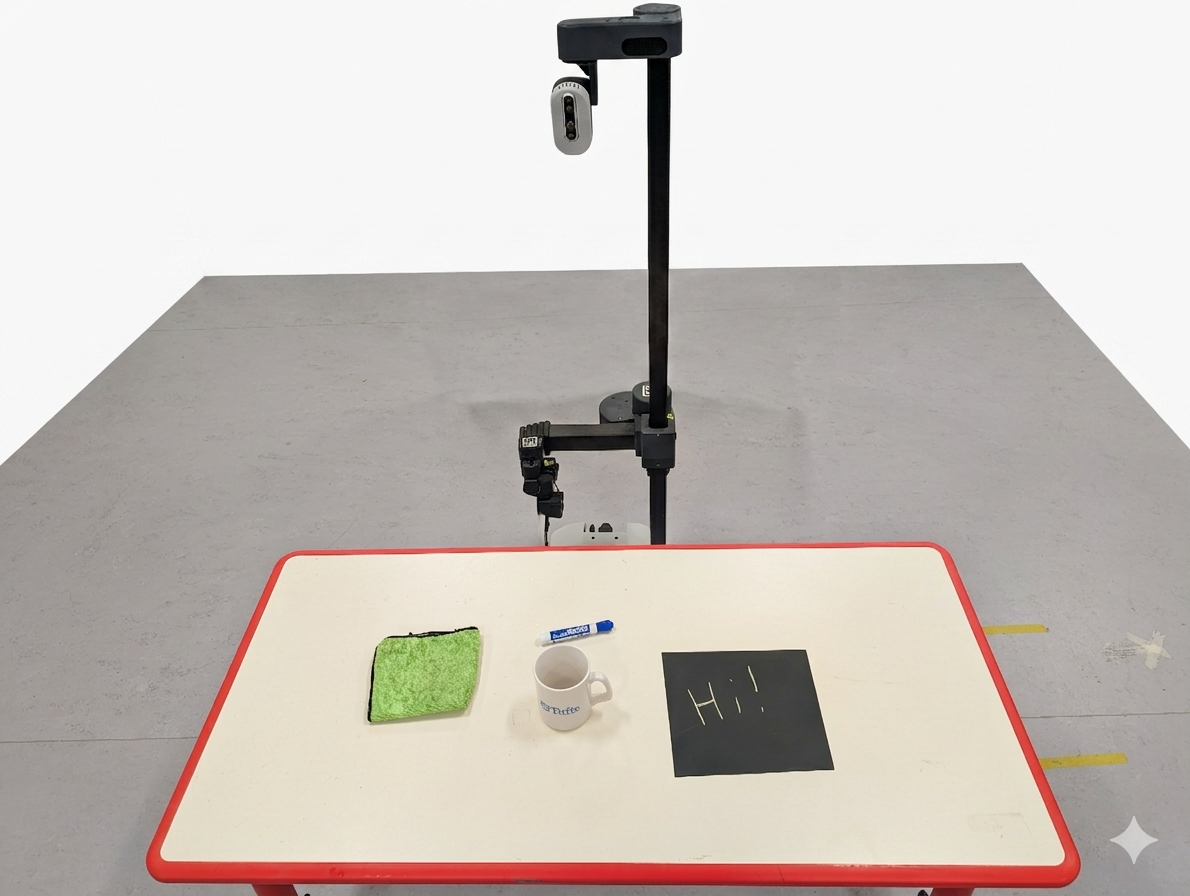
\includegraphics[width=3cm]{figures/robot_photo.png}\\[1pt]Physical Task};

    % right column: the two PDDL stages, placed RELATIVE to the photo
    % (fixed gap) so font-metric differences never cause overlap
    \node[stage,anchor=north west] (rt) at ([xshift=1.1cm]photo.north east) {%
      \begin{tabular}{@{}c@{}}
        {\footnotesize\bfseries\color{accent} Runtime Generated PDDL} {\scriptsize (with Typing Gap)}\\[1pt]
        \pddlpanel{Typed Domain}{\usebox\pddlDomA}\\[1pt]
        \pddlpanel{Untyped Problem}{\usebox\pddlProbU}
      \end{tabular}};
    % The domain is unchanged by the LLM (only the problem's object types are
    % repaired), so it is shown once above; this stage shows just the repaired problem.
    \node[stage,anchor=north,below=0.4cm of rt] (ll) {%
      \begin{tabular}{@{}c@{}}
        {\footnotesize\bfseries\color{accent} LLM Typed PDDL} {\scriptsize (Repaired Problem)}\\[1pt]
        \pddlpanel{Typed Problem}{\usebox\pddlProbT}
      \end{tabular}};

    % left column: remaining actors, spread to match right-column height
    \node[bigbox,anchor=south] (planner) at (photo.south |- ll.south)
        {
\includegraphics[width=1.15cm]{figures/icon_planner.png}\\[1pt]Symbolic Planner};
    \node[bigbox] (llm) at (photo.south |- {$(rt.south)!0.5!(ll.north)$})
        {
\includegraphics[width=1.1cm]{figures/icon_llm.png}\\[1pt]CAST LLM\\Preprocessing};

    % zig-zag flow: photo -> rt -> llm -> ll -> planner -> photo.
    % The LLM's incoming and outgoing arrows both attach at (llm.east) with
    % mirror-image arcs so they read as a single pass-through point.
    \draw[flow] (photo.east) -- (photo.east -| rt.west);
    \draw[flow] (rt.west)  to[out=180,in=0] (llm.east);
    \draw[flow] (llm.east) to[out=0,in=180] (ll.west);
    \draw[flow] (ll.west)  to[out=180,in=0] (planner.east);
    % feedback loop routed around the far left, clear of the LLM box
    \coordinate (FL) at ([xshift=-0.55cm]photo.west);
    \draw[flow] (planner.west) -- (planner.west -| FL)
          -- (photo.west -| FL) -- (photo.west);
  \end{tikzpicture}}
  \caption{\small{The CAST typing pipeline. A physical task is encoded at runtime into a typed domain and a problem whose objects carry only an overly-general base type, leaving the goal unreachable (the typing gap). The LLM reassigns each object a functional type already defined in the domain (highlighted), and the repaired problem is handed to a symbolic planner.}}
    \label{fig:robot_example}
\end{figure}

\section{Introduction}
\label{sec:intro}
Robots deployed in open-world environments must operate under conditions that
cannot be fully anticipated at design time~\cite{wray2025requirements}. Expected tools may be missing,
unfamiliar objects may be present, and the available resources may support ways
of completing a task that were not encoded in advance. Reliable autonomy
therefore requires some capacity to adapt to the current environment without
giving up the structure and predictability needed to understand and verify the
robot's behavior.

Symbolic task planners provide this structure by reasoning over explicit models
of objects, actions, and their effects \cite{mcdermott1998pddl}. However, their
ability to find a plan depends on the environment being represented in the
planner's predefined vocabulary. A runtime perception system may recognize
objects such as a \texttt{cloth}, \texttt{cup}, and \texttt{marker}, while the
planning domain defines actions over functional types such as
\texttt{eraser}, \texttt{container}, and \texttt{writing-tool}. When no
available object is assigned the type required by an action, planning fails
even when an object in the environment could fulfill the required role.

% Classic task planner provide systematic search and formal criteria for plan validity once the world has been expressed in a symbolic planning language such as PDDL~\cite{mcdermott1998pddl}. In open worlds, however, constructing this representation is itself a substantial challenge. A runtime perception
% system may recognize objects such as a \texttt{cloth}, \texttt{cup}, and
% \texttt{marker}, while the planning domain defines actions over functional
% types such as \texttt{eraser}, \texttt{container}, and \texttt{writing-tool}.
% When no perceived object is assigned the type required by an action, grounding
% excludes that action and planning fails---even when an available object could
% fulfill the required role. In such cases, the environment contains a solution,
% but the symbolic problem does not represent it.

Consider a robot asked to clean a whiteboard when no conventional eraser is
present. A cloth may provide the required wiping function, but a typed planner
cannot use it if the cloth is represented only as a generic graspable object.
We call this mismatch between the available objects and the goal-relevant type
requirements of the planning domain a \emph{typing gap}. Typing gaps can arise
when problem instances are generated from open-vocabulary perception, when
object annotations are incomplete, or when a hand-authored object-to-type
mapping cannot anticipate every functionally appropriate object that may be
encountered at runtime. Resolving such a gap does not necessarily require
inventing a new action or changing the task. It may be sufficient to recognize
that an available object can instantiate an existing symbolic role.

In this work, we focus on one bounded form of such adaptation: determining
whether an object already present in the environment can fulfill a functional
role required by one of the robot's existing skills. We do not expand the
robot's action repertoire or relax the task. Instead, we revise how available
objects are typed so that the symbolic planner can consider functionally
appropriate alternatives.

Large language models provide semantic knowledge that can support functional
substitution, but remain unreliable as end-to-end generators of symbolic plans~\cite{valmeekam2023planbenchextensiblebenchmarkevaluating, Stein_Fišer_Hoffmann_Koller_2025}. We therefore position the
LLM upstream of the planner, using it to adapt the symbolic representation
rather than to generate actions.

We introduce CAST, \textbf{C}onstrained \textbf{A}ssignment of \textbf{S}ymbolic \textbf{T}ypes, which uses an
LLM to assign available objects to types already defined in the planning
domain. The resulting problem is then passed to an off-the-shelf symbolic
planner, which remains responsible for generating the final plan. This
separation allows the system to benefit from the LLM's semantic knowledge while
retaining the structure of symbolic planning.

We investigate three CAST variants: consensus voting, iterative refinement,
and judge-based selection, and evaluate their ability to recover valid plans,
refuse problems for which no suitable substitute exists, and manage inference
costs. Across multiple problem configurations and semantic variations, CAST
substantially outperforms both an end-to-end LLM planning baseline and an
unconstrained baseline that lets the LLM rewrite the PDDL directly, on tasks
requiring functional substitution. We additionally demonstrate the complete pipeline on
a physical robot.


% \section{Introduction}

% Classic task planner provide systematic search and formal criteria for plan validity once the world has been expressed in a symbolic planning language such as PDDL~\cite{mcdermott1998pddl}. In open worlds, however, 

% Robots are increasingly moving beyond controlled laboratory settings into open-world environments. In these settings, they must contend with environmental novelties, including unexpected objects, missing tools, and previously unseen task configurations. Adapting to such novelty is essential for reliable long-horizon autonomy. However, adaptation alone is insufficient: deployable robotic systems must also remain explainable and verifiable so that their behavior can be trusted and their decisions understood~\cite{jones2026requirements, wray2025requirements}.

% Symbolic task planners provide strong guarantees of soundness and completeness, making them attractive for trustworthy robot autonomy. However, these guarantees rely on closed-world assumptions in which object types, predicates, and actions are fully specified. Consequently, planning fails whenever required object types are unavailable, even if functionally equivalent alternatives exist in the environment. 
% Recent work has sought to address this limitation using large language models (LLMs). Methods such as AutoPlanBench ~\cite{Stein_Fišer_Hoffmann_Koller_2025} generate plans directly from symbolic task descriptions, leveraging the semantic knowledge encoded in LLMs to improve flexibility. However, because the learned model is responsible for producing the final plan, hallucinations and reasoning errors directly affect execution, resulting in plans that may be invalid, unsafe, or unverifiable.

% Consider a robot instructed to erase a whiteboard. A symbolic planner expects an object of type \texttt{eraser}, but none is present in the environment. Although a cloth or tissue could fulfill the same functional role, the planner cannot infer this substitution because the object types are fixed in the planning domain. Conversely, an LLM may correctly recognize a cloth as a substitute, but it may also incorrectly suggest an object such as a brick. Effective adaptation therefore requires a mechanism that can leverage semantic knowledge while rejecting invalid substitutions and preserving the guarantees of symbolic planning.

% Rather than placing the LLM in charge of generating the final plan, we position it upstream of the symbolic planner. We propose \textsc{CAST} (Constrained Assignment of Symbolic Types), a framework that leverages an LLM to dynamically assign symbolic types to objects at runtime, bridging the gap between the objects available in the environment and the type requirements of the planning domain. By restricting the LLM to modifying the symbolic problem representation rather than generating actions directly, \textsc{CAST} preserves the symbolic planner as the sole plan-generation component. Consequently, every generated plan remains subject to the planner's soundness and completeness guarantees while benefiting from the LLM's semantic knowledge to resolve environmental novelty. We evaluate three querying strategies—consensus voting, iterative refinement, and judge-based selection—across two open-weight models, measuring their ability to identify valid substitutions and appropriately refuse tasks for which no suitable substitute exists. We further compare \textsc{CAST} against AutoPlanBench, an existing LLM-based planning benchmark.

% The contributions of this work are threefold:
% We introduce CAST, a framework for runtime symbolic type assignment that enables symbolic planners to adapt to missing object types.
% We investigate three LLM querying strategies and evaluate their ability to both identify valid substitutions and appropriately refuse impossible substitutions.
% We compare CAST against AutoPlanBench across multiple domains and demonstrate that separating semantic adaptation from symbolic planning substantially improves planning robustness while preserving planner guarantees.

% Symbolic planners offer soundness and completeness guarantees, but are rigid by design: they assume closed-world representations of objects and the actions that apply to them, and fail outright when a required object type is absent. Approaches that include generative models trade these guarantees for flexibility. These systems include LLM-as-planner methods such as AutoPlanBench~\cite{Stein_Fišer_Hoffmann_Koller_2025} that generate plans directly from PDDL. They introduce flexibility through approximation, but because the learned component produces the plan itself, its failures propagate directly into the output: hallucination and flawed reasoning can lead to unsafe and incorrect plans with no guarantee of validity.

% Consider the task of erasing a whiteboard, where at deployment time, the agent has no access to an eraser-typed object. In this situation, if a functionally equivalent object such as a cloth is present in the environment, the agent should be able to update its representation to substitute, without causing any issues 

% If no \texttt{eraser}-typed object is present in the problem definition, a symbolic planner cannot yield a solution --- even when a functionally equivalent substitute, such as a cloth or tissue, might be available in the environment. For example, an incompatible object such as a brick could be selected by an LLM, producing a plan that is unsafe or simply wrong.
% Using an LLM trained on a large-scale internet data, this information can easily be captured. However, the LLMs risk the verifiability, and are prone to hallucinations. 
% Adapting to novelties therefore demands not only proposing substitutions, but also refusing them when no valid option exists.

% Rather than placing the LLM component in charge of generating a final plan, we place it upstream of the planner. We propose \textsc{CAST} (Constrained Assignment of Symbolic Types), which leverages an LLM to dynamically assign types to objects at runtime, resolving the gap between the available objects and the type requirements of a symbolic planner. Because the LLM only shapes the representation the planner consumes, and does not generate the plan, we realize the flexibility of a learned approach without sacrificing the planner's completeness guarantees. We evaluate three querying strategies (consensus voting, iterative refinement, and judge-based selection) across two open-weight models, benchmarking their ability to correctly resolve object substitutions and appropriately refuse problems for which no valid substitute exists. We further compare against AutoPlanBench, an existing LLM-based planning benchmark.

% Our results show that typing-based approaches significantly outperform the LLM-based planning baseline on problems requiring substitution. We benchmark across problems of varying complexity and semantic variation, demonstrating robustness to differences in object naming across domains. We further find that the choice of querying strategy introduces a trade-off: approaches that maximize successful plan generation on solvable problems tend to be more willing to produce plans even when no valid substitute exists, while more conservative strategies are better at declining to plan altogether.



% On the other spectrum, completely relyung on an LLM as a planning repair syste,
% Simply because the object cannot be classified as that type on-the-fly. 
% A learned system may recognize this substitution, but large models are prone to hallucination: for example, an incompatible object such as a brick could be selected by an LLM, producing a plan xthat is unsafe or simply wrong.
\section{Related Work}
\subsection{Model Repair in Symbolic Planning}
Creative problem solving can be described as a failure in an agent's
understanding of the world such that it is insufficient to complete a
given task \cite{ijcai2023p777}. Existing literature has explored
various approaches to this problem. In one line of work reinforcement
learning (RL) is used to discover action primitives after reaching an
unrecoverable state \cite{rapid_learn, lorang_rsj_2024}. \citet{gizzi_ieee_2019}
propose a system that enumerates action-object combinations after
reaching a failure case. Rather than learning
entirely new action primitives or having to test many different
action-object pairs, our approach seeks to use an LLM to offer object
substitions.

Repair approaches address planning tasks that are unsolvable as specified, asking how the specification can be modified so that a solution exists~\cite{bercher2025modelrepair}. \citet{gragera2023repair}, for example, perform repair by fixing incomplete action effects by compiling the unsolvable task into an extended task that may insert the missing effects. Our approach instead works by reassigning the types of objects already present in the problem, leaving the domain, goal, and initial state intact. Most relevant to our design, \citet{gragera2023exploring} prompt an LLM \emph{stand-alone} to fix unsolvable tasks and find its limited reasoning insufficient for identifying repairs that yield solvable tasks. We reach a different outcome by changing the LLM's role: rather than trusting it to repair the task, we confine it to proposing type reassignments and delegate all verification to the symbolic planner.

\subsection{LLMs for Planning}
The use of LLMs for symbolic planning has been widely explored, with
mixed results. \citet{motwani2026longcot} find that LLMs struggle with long-horizon Chain of Thought (CoT) tasks in general. Benchmarking that uses LLMs for plan generation confirms that LLMs do not reliably produce correct plans
\citep{valmeekam_large_nodate, valmeekam2023planbenchextensiblebenchmarkevaluating}. Despite these limitations, LLMs have shown promise as components within larger planning pipelines rather than as end-to-end planners. \citet{liu_llmp_2023} use LLMs to generate PDDL problem files from natural language descriptions, while \citet{singh_twostep_2024} demonstrate that LLMs can decompose problems into simpler sub-tasks amenable to parallel execution. Researchers have similarly integrated LLMs into Hierarchical Task Networks to break high-level goals into more tractable sub-tasks \citep{pmlr-v288-munoz-avila25a, xu2025online}. LLMs have also been used to find symbolic models given pre-existing black-box style executors \cite{yang2026skillwrappergenerativepredicateinvention}.

Another line of research uses LLM-generated outputs to guide or improve
search and learning. \citet{silver2022pddl} propose treating an LLM-generated
plan, even an incorrect one, as a heuristic to guide greedy
best-first search, and \citet{hazra_saycanpay_2024} similarly incorporate heuristics to improve LLM-based planning. \citet{kambhampati_llms_2024} take a complementary
approach, employing critics to evaluate and refine plans produced by
LLMs. Researchers have also explored
using LLMs' code generation capabilities to produce programs that
solve specific tasks \citep{silver2024generalized}.

Prior research has also explored using LLMs to create symbolic representations of the world at runtime \cite{argenziano2024empowerembodiedmultiroleopenvocabulary}. Most closely related to our own work, \citet{musumeci2025context} propose using an LLM to generate and iteratively refine PDDL, combined with a symbolic planner to find suitable goal substitutions when the original goal is not reachable. In contrast, our approach preserves the original goal by using an LLM to reclassify available objects into the required types at runtime, enabling the original plan to remain valid without relaxing the task specification.
\section{Preliminaries}

\subsection{Symbolic Planning}
\subsubsection{Classical Planning with Types}

% We adopt the PDDL planning formalism~\cite{mcdermott1998pddl}, which extends classical STRIPS~\cite{fikes1971strips} with a type hierarchy. A planning domain $D$ consists of a set of predicates $\mathcal{P}$, a set of actions $\mathcal{A}$, and a type hierarchy $\mathcal{T}$. Each type $\tau \in \mathcal{T}$ denotes a set of objects; the hierarchy imposes $\tau_1 \sqsubset \tau_2$ (e.g., $\texttt{eraser} \sqsubset \texttt{tool} \sqsubset \texttt{object}$). Each action $a \in \mathcal{A}$ is defined as $a = \langle \text{pre}(a), \text{add}(a), \text{del}(a) \rangle$ where $\text{pre}(a), \text{add}(a), \text{del}(a) \subseteq \mathcal{P}$, and each parameter of $a$ is constrained to a type $\tau \in \mathcal{T}$. A planning problem $\Pi = (D, O, \sigma, I, G)$ pairs the domain with a set of objects $O$ and a type assignment $\sigma : O \rightarrow \mathcal{T}$. Let $\mathcal{F}$ denote the set of ground atoms obtained by instantiating the predicates $\mathcal{P}$ with objects from $O$. A \emph{state} $s \subseteq \mathcal{F}$ is a set of ground atoms; the initial state $I \subseteq \mathcal{F}$ is one such state, and the goal $G \subseteq \mathcal{F}$ is a set of atoms defining the \emph{goal states} $\{\, s \mid G \subseteq s \,\}$. The type assignment $\sigma$ determines action applicability: an action schema parameterised over type $\tau$ may only be grounded with objects $o$ such that $\sigma(o) \sqsubseteq \tau$.

% A \textit{plan} $\pi$ is a sequence of grounded actions $\langle a_1, \ldots, a_k \rangle$ such that executing the sequence from $I$ satisfies $G$. A symbolic planner takes $\pi$ as input and returns either a valid plan or reports that no plan exists.


We adopt the typed STRIPS fragment of the Planning Domain Definition Language (PDDL)~\cite{mcdermott1998pddl}, which extends classical STRIPS~\cite{fikes1971strips} with typed objects and action parameters. A planning domain $D = \langle \mathcal{P}, \mathcal{A}, \mathcal{T}, \sqsubseteq \rangle$ consists of predicate symbols $\mathcal{P}$, action schemas $\mathcal{A}$, types $\mathcal{T}$, and a reflexive subtype relation $\sqsubseteq$ (e.g., $\texttt{eraser} \sqsubseteq \texttt{tool} \sqsubseteq \texttt{object}$). Each action schema $a \in \mathcal{A}$ is a tuple $a = \langle \mathrm{par}(a), \mathrm{pre}(a), \mathrm{add}(a), \mathrm{del}(a) \rangle$, where $\mathrm{par}(a)$ are typed parameters and the remaining components are sets of atoms over those parameters. Preconditions are positive conjunctions, and effects are represented by add and delete lists.

A planning problem $\Pi = \langle D, O, \sigma, I, G \rangle$ consists of a domain $D$, a finite set of objects $O$, a type assignment $\sigma : O \rightarrow \mathcal{T}$, an initial state $I$, and a goal $G$. Let $\mathcal{F}$ be the set of all well-typed ground atoms over $\mathcal{P}$ and $O$. A state $s \subseteq \mathcal{F}$ contains the atoms true in that state, while omitted atoms are false under the closed-world assumption. The initial state $I \subseteq \mathcal{F}$ is a single fully specified state, whereas $G \subseteq \mathcal{F}$ defines the goal-state set $S_G = \{\,s \subseteq \mathcal{F} \mid G \subseteq s\,\}$.

A parameter of type $\tau$ may be grounded with an object $o$ only if $\sigma(o) \sqsubseteq \tau$. A well-typed grounded action $a$ is applicable in $s$ if $\mathrm{pre}(a) \subseteq s$, and produces the successor state $\gamma(s,a) = (s \setminus \mathrm{del}(a)) \cup \mathrm{add}(a)$. A plan for $\Pi$ is a finite sequence of well-typed grounded actions $\rho = \langle a_1,\ldots,a_k\rangle$ that are successively applicable and satisfy $G \subseteq \gamma(I,\rho)$. A sound and complete symbolic planner takes $\Pi$ as input and returns a valid plan if one exists, or establishes that no plan exists.

\label{sec:preliminaries}

\subsection{Running Example}
Consider the task depicted in Figure~\ref{fig:robot_example}. The environment consists objects $\mathcal{O} = \{\mathtt{marker}, \mathtt{cloth}, \mathtt{cup}, \mathtt{blackboard}\}$. The robot's task is to wipe the blackboard, and it has actions $\mathcal{A} = \{\mathtt{wipe}, \mathtt{pickup} \}$. 

% We also assume the same formalisms defined in the Symbolic Planning section. Therefore, 
The actions and objects possess types which restricts the number of grounded actions generated for each lifted action encoding. For example, an object can be typed as \texttt{pickable}, which simply categorizes objects that can be assigned to the \texttt{pickup} action. Let us assume that these types correspond to the object names listed in $\mathcal{O}$. In the example, no object of type \texttt{eraser} is present, so a plan would not be able to be generated. However, in this example a different object, \texttt{cloth} could be used in place of an \texttt{eraser}. 
 

% For example, the \texttt{wipe} action can encode that an object of the type \texttt{eraser} can be used to erase an object of the type \texttt{blackboard}. Each object would also be assigned a type, let us assume that these types correspond to the object names listed in $\mathcal{O}$.

% We consider two ways the the set of object can be generated:  they may be manually added to the problem file, or the problem file might be generated at run time using the robots sensors such as camera. In the case where a hand crafted problem file is available, objects must be annotated with labels that allow the planner to determine which actions can be applied to which objects. This requires a comprehensive list of types, and additionally may not encode different ways of solving the problem apriori. In the other scenario where the problem file is generated from sensor observations - it is important to consider how types can be associated with each object. In the most general sense, a problem file can be generated assigning each object to a generic type, however this would allow for plans like using the `cup` to clean the `blackboard`, which is not reasonable.


\subsubsection{The Typing Problem}

A \textit{typed domain} $D_t$ encodes affordances via type constraints: for example, \texttt{wipe} requires an $\texttt{eraser}$-typed tool and a $\texttt{whiteboard}$-typed surface. In practice, objects such as \texttt{cloth} may be assigned only the base type $\texttt{tool}$ --- either because the problem was constructed at runtime from untyped perception, or because a fixed object-to-type mapping is unavailable. An object typed at $\texttt{tool}$ is ineligible for any action whose parameter requires $\texttt{eraser}$, even if that object could functionally serve the role. Not every object in $O$ requires reassignment --- objects already typed at an appropriate subtype, or irrelevant to the goal's action chain, retain their types under $\sigma$.

Crucially, the goal $G$ determines which types are required; for example to achieve $\texttt{(clean blackboard)}$, the planner must execute $\texttt{wipe}$, which requires an $\texttt{eraser}$-typed object. Observe that properties irrelevant to this action chain, such as an objects $\texttt{color}$ ,need not be typed. When $\sigma$ assigns objects to insufficient types, the grounded action space is such that no plan achieving $G$ exists. We call this a \textit{typing gap}. A typing gap is a restricted instance of \emph{model repair}~\cite{bercher2025modelrepair}: the only modification permitted is reassignment of object types, leaving the domain, goal, and initial state untouched.

\subsubsection{Failure Modes}

Given a typed domain $D_t$ and a problem instance with a typing gap, there are two distinct failure cases. First, a valid substitution may exist --- some object in $O$ could plausibly fill the required subtype --- but the type assignment $\sigma$ fails to reflect this. Second, no object in $O$ is a plausible instance of the required subtype: no valid substitution exists and the correct behavior is to return no plan.

\subsection{Large Language Model Queries}
\label{subsec:llm_query}

Given a prompt $\rho$ encoding a planning domain $D$ and problem $\pi$, a large language model $L$ returns a proposed type assignment $\hat{\sigma} : O \rightarrow \mathcal{T}$, expressed as a set of pairs $\{(o, \tau) \mid o \in O,\, \tau \in \mathcal{T}\}$. Since $L$ is a stochastic function, repeated queries over the same $\rho$ may yield different assignments. The goal of LLM-based typing is to find a $\hat{\sigma}$ that resolves the typing gap in $\pi$, enabling a symbolic planner to return a valid plan.

\subsection{Problem Formulation}

Given a problem $\pi$ exhibiting a typing gap, our objective is to find a type assignment $\hat{\sigma}$ under which the planner returns a plan achieving $G$, or to correctly report that no valid substitution exists. Every strategy in the next section instantiates the same template: an LLM proposes one or more candidate assignments $\hat{\sigma}$, and each is verified by invoking the symbolic planner on $\pi|_{\hat{\sigma}}$. Because verification is delegated to the planner rather than the LLM, the framework inherits the planner's guarantees relative to the assigned types.

While we retain the planner's formal guarantees, this is not to say the approach is without a trade-off. In exchange for the flexibility to solve problems a rigid planner would declare unsolvable, we give up any guarantee on the \emph{semantic} validity of $\hat{\sigma}$ --- whether a substitution such as \texttt{cloth}-as-\texttt{eraser} is physically warranted. The planner cannot certify this; it is precisely what our experiments serve to measure.
\section{Methodology}

We present our three LLM querying strategies for resolving typing gaps at runtime. Each strategy represents different trade-offs between token cost, flexibility, and robustness. All three approaches share a common structure: given an untyped or partially typed PDDL problem, an LLM is queried to assign types to available objects, and the resulting typed problem is passed to a symbolic planner. They differ in how the LLM is queried, how feedback is incorporated, and how disagreement is resolved.

\subsection{Consensus Based Typing}

\begin{algorithm}[t]
  \caption{CAST: Consensus Variant}
  \label{alg:consensus-typing}
  \begin{algorithmic}[1]
    \footnotesize
    \Require domain $D$, problem $\Pi=\langle O,I,G\rangle$, LLM, planner, number of queries $n$, prompt $\rho_T$
    
    \State $\mathcal{Q} \gets [ \,]$
    
    \For{$i = 1$ to $n$} 
      \State $\mathcal{Q}.\mathrm{append}(L(D, \Pi, \rho_T))$ \Comment{collect candidate $\hat{\sigma}$}
    \EndFor
    
    \State $\mathrm{votes}(o,\tau) \gets |\{i \in \mathcal{Q} : i(o) = \tau\}|$ for $o \in O,\, \tau \in \mathcal{T}$
    \State $\hat{\tau}(o) \gets \arg\max_{\tau} \mathrm{votes}(o,\tau)$ for $o \in O$
    \State $A_o \gets [\tau \mid \mathrm{votes}(o,\tau) > 0]$ sorted by $\downarrow$ votes

    \For{each $o \in O$ with $|A_o|>1$, sorted $\uparrow$ by vote share}
      \For{each $\tau \in A_o$} \Comment{every candidate type for $o$}
        \State $\tau' \gets \hat{\tau}$ with $o \mapsto \tau$ \Comment{relax $o$ to candidate type $\tau$}
        \State $\pi \gets Planner(D, \Pi|_{\tau'})$
        \If{$\pi \neq \emptyset$}
          \State \Return $\pi$
        \EndIf 
      \EndFor 
    \EndFor
    
    \State \Return $\emptyset$
  \end{algorithmic}
\end{algorithm}

The consensus-based approach exploits the stochastic nature of LLMs: repeated queries over the same prompt may yield distinct type assignments. By querying the LLM $n$ times, we build a distribution of votes over mappings between each object $o$ and candidate types $\tau \in \mathcal{T}$. Algorithm~\ref{alg:consensus-typing} formalises this approach. The LLM generates $n$ candidate assignments $\hat{\sigma}$, from which a majority-vote assignment $\hat{\tau}$ is derived by selecting the most-voted type per object. The planner is first attempted under $\hat{\tau}$; if a plan is found, we terminate. Otherwise, for each object with type disagreement across queries, we substitute alternative types one object at a time. This keeps all others at their majority type, in ascending order of vote share. We then attempt the planner after each substitution and return the first plan found. If no substitution yields a solution, we return an $\emptyset$. This recovery explores only single-object relaxations of the majority assignment; problems that require several objects to be simultaneously re-typed beyond the majority vote are outside the scope of this relaxation step.


\subsection{Iterative and Judge Typing}
\begin{algorithm}
  \caption{CAST: Iterative / Judge Variant}
  \label{alg:iterative-judge}
  \begin{algorithmic}[1]
    \footnotesize
    \Require domain $D$, problem $\Pi=\langle O,I,G\rangle$, LLM, planner, max iterations $T$, prompt $\rho_T$; judge mode also uses Judge and prompt $\rho_J$

    \State $f \gets \texttt{null}$ \Comment{no feedback on first call}

    \For{$t = 1$ to $T$}
      \State $\hat{\sigma} \gets L(D, \Pi, \rho_T, f)$
      \If{\textbf{judge mode}}
        \State $j \gets Judge(D, \Pi, \hat{\sigma}, \rho_J)$
        \If{$j.\mathrm{approved}$} \textbf{break} \Comment{plan below}
        \EndIf
        \State $f \gets j.\mathrm{feedback}$
      \Else \Comment{iterative mode}
        \State $\pi \gets Planner(D, \Pi|_{\hat{\sigma}})$
        \If{$\pi \neq \emptyset$} \Return $\pi$ \Comment{solved}
        \EndIf
        \State $f \gets \mathrm{PlannerFeedback}(\hat{\sigma},\, t,\, T)$
      \EndIf
    \EndFor

    \If{\textbf{judge mode}}
      \State \Return $Planner(D, \Pi|_{\hat{\sigma}})$ \Comment{plan on final $\hat{\sigma}$}
    \EndIf
    \State \Return $\emptyset$ \Comment{iterative: no plan within budget}
  \end{algorithmic}
\end{algorithm}

Unlike consensus, which always issues exactly $n$ queries, the iterative and judge strategies (Algorithm~\ref{alg:iterative-judge}) both re-query the LLM with feedback and can succeed in as few as one query, repeating for at most $T$ iterations. They differ only in what validates a proposed assignment $\hat{\sigma}$. \emph{Iterative} typing invokes the planner directly: on failure, it re-queries the LLM with feedback and returns the first plan found, or $\emptyset$. \emph{Judge} typing instead interposes a judge call to the same LLM, prompted differently via $\rho_J$, that evaluates $\hat{\sigma}$ semantically before any planning; if approved, the loop exits and the planner is invoked once on that assignment; if it fails, judge typing returns $\emptyset$ rather than resuming refinement. Otherwise, the judge's feedback drives another round of typing. The distinction is where the loop is closed: iterative is guided by planner failure, whereas judge filters semantically poor assignments before planning is attempted at all. It never revisits an assignment the judge has already approved.

Both methods utilize feedback to re-query the LLM upon failure; however, the content of the feedback varies. For iterative typing it may be as simple as a boolean planner-failure signal; our implementation returns the previous object-to-type assignments alongside the failure and instructs the LLM to reconsider $\hat{\sigma}$. The judge is prompted to reason at a high level about whether goal-relevant objects are correctly typed and whether the assignment is likely solvable; if none is approved within budget, the planner is run on the final proposal as a fallback.


\section{Experiments}
\subsection{Environments}
% Standard planning benchmarks, including those from the International Planning Competition (IPC), primarily evaluate planning performance under a correctly specified symbolic model. 
% They vary complexity through larger search spaces and grounding complexity, but generally assume that objects are already assigned appropriate symbolic types. 
Standard planning benchmarks, such as those from the International Planning Competition (IPC), are designed to evaluate planner performance by increasing search-space size and grounding complexity. By construction, however, they assume a correctly specified type assignment: objects required by relevant actions are already assigned appropriate symbolic types. They therefore do not evaluate the capability studied here—identifying and repairing \emph{typing gaps} at runtime. To evaluate this capability directly, we construct a benchmark that systematically introduces typing gaps while holding the underlying planning structure fixed. This design separates type-repair performance from search difficulty and isolates the LLM's ability to identify available objects that can fulfill the required symbolic roles.

% Standard planning benchmarks, such as those from the International Planning
% Competition (IPC), are constructed to stress the \emph{planner}: they scale search
% and grounding complexity but, by design, contain no \emph{typing gap} (i.e., every
% object needed by the required action is already correctly typed), so they cannot
% exercise the capability we study.
% Because the gap is a property of the representation rather than of the search, we introduce a benchmark that induces typing gaps directly while holding planning structure fixed, isolating the variable of interest: the LLM's ability to recognize functional equivalence.

% Our base domain, \emph{construction}, consists of a single domain file with the actions $\mathcal{A} = \{$\texttt{smash-cover} (tool:\texttt{hammer}, fastener:\texttt{fastener}), \texttt{hit-nail}(tool:\texttt{hammer}, fastener:\texttt{nail}), \texttt{turn-bolt}(tool:\texttt{wrench}, fastener:\texttt{bolt}), \texttt{turn-screw}(tool:\texttt{screwdriver}, fastener:\texttt{screw})$\}$. In every problem, the canonical tool is absent, opening a typing gap that a functionally equivalent substitute present in the environment must close.

Our base domain, \emph{construction}, defines four actions: \texttt{smash-cover}(\texttt{tool: hammer}, \texttt{fastener: fastener}), \texttt{hit-nail}(\texttt{tool: hammer}, \texttt{fastener: nail}), \texttt{turn-bolt}(\texttt{tool: wrench}, \texttt{fastener: bolt}), and \texttt{turn-screw}(\texttt{tool: screwdriver}, \texttt{fastener: screw}). Each problem omits the canonical tool required by the goal-relevant action, thereby creating a typing gap. Solvable instances contain a functionally appropriate alternative whose initial type prevents the planner from using it, whereas no-substitution instances contain no valid alternative.

To broaden our evaluation, we additionally construct a family of alternative domains. Using Claude Sonnet 4.6, we generate four domains --- \emph{medic}, \emph{kitchen}, \emph{electronics}, and \emph{survival}. Each domain uses entirely different actions, types, predicates, and object vocabularies, such as \texttt{incise-wound} with a \texttt{scalpel} or \texttt{dice-vegetable} with a \texttt{chef-knife}. Structurally, however, each is a
pure lexical relabeling of \emph{construction}: the number of actions, their arities, and the number of types, predicates, and goals are all identical --- only the surface names differ. Because the domains have identical planning structures, performance differences indicate how reliably the LLM recognizes functional substitutes in different semantic contexts, rather than differences in planning complexity.


% To probe how substitution behavior depends on \emph{semantics} rather than
% \emph{structure}, we additionally construct a family of lexically distinct but
% structurally isomorphic domains. We prompt Claude Sonnet 4.6, to generate four
% alternative domains --- \emph{medic}, \emph{kitchen}, \emph{electronics}, and
% \emph{survival} --- each with entirely different actions, types, predicates, and
% object vocabularies (e.g., \texttt{incise-wound} with a \texttt{scalpel}, or
% \texttt{dice-vegetable} with a \texttt{chef-knife}), but with a planning skeleton
% identical to construction: the same number of roles, actions, and goals, and the
% same single-substitution dependency structure. Any performance difference therefore isolates the LLM's cross-domain functional knowledge, free of confounds from planning difficulty.


\subsection{Evaluation Framework}
\label{subsec:eval_framework}
\paragraph{Problem Configurations}
We organize the benchmark problems into four categories that vary the number of required substitutions, the number of distractor objects, and whether a valid substitution exists:

\begin{itemize}\item \textbf{Single} The canonical tool required to achieve the goal is absent, but one available object can serve as a valid functional substitute. Solving the problem requires one object-to-type reassignment. \textit{RQ1: Can CAST identify a valid substitute when the canonical tool is absent?}

\item \textbf{Bulk} The goal contains multiple components that require several substitutions simultaneously. A plan can be found only if all required objects are assigned appropriate functional types. \textit{RQ2: How does CAST perform when several substitutions are required simultaneously?}

\item \textbf{Stress} A single-substitution problem is augmented with 10, 20, or 50 distractor objects that cannot validly fulfill the required role. \textit{RQ3: How robust is CAST as the number of distractor objects increases?}

\item \textbf{No Substitution} The canonical tool is absent, and none of the available objects can validly fulfill the required role. The correct outcome is therefore to leave the typing gap unresolved and return no plan. \textit{RQ4: Does CAST correctly refuse to produce a plan when no valid substitute exists?}
\end{itemize}

We additionally evaluate the single-substitution configuration across the four structurally matched semantic domains described above. \textit{RQ5: Does substitution performance remain robust when the same planning structure is expressed in different semantic contexts?}




% \begin{itemize}
% \item \textbf{Single} -- A handful of tools and a goal where the
%   tool traditionally used to solve the goal is missing. One of the
%   available tools can be validly substituted to solve the goal (e.g.,
%   substituting a tool as a hammer to drive in a loose
%   nail). \textit{RQ1:} \textit{Can the LLM correctly identify a valid tool
%   substitution when the canonical tool is absent?}
% \item \textbf{Bulk} -- A modification of single where the goal
%   consists of multiple parts, requiring multiple
%   substitutions. \textit{RQ2:} \textit{Does substitution accuracy degrade as
%   the number of simultaneous goals increases?}
% \item \textbf{Stress} -- A modification of standard with many
%   additional distractor tools, designed to test how the LLM scales
%   when reasoning over a larger set of objects. \textit{RQ3:} \textit{How does
%   substitution accuracy scale as the number of distractor objects
%   grows?}
% \item \textbf{No Substitution} -- Impossible problems where no valid
%   substitution exists among the available tools, rendering the task
%   unsolvable. \textit{RQ4:} \textit{Does the LLM avoid false positives when no
%   valid substitution exists?}
% \end{itemize}

% Beyond these categories, the isomorphic synonym domains introduced above probe semantic robustness. \textit{RQ5:} Is substitution accuracy robust when the same structural task is re-expressed in an unrelated semantic domain?

% All problems are accompanied by hand-annotated lists of valid substitutions, which ensure that the LLM does not assign unreasonable types (e.g., a napkin cannot reasonably be used to hammer in a nail). Every returned plan $\pi = \langle a_1,\ldots,a_k\rangle$ is independently re-verified by applying its actions in sequence from the initial state and confirming that the resulting state satisfies the goal $G$; we additionally check the plan against the hand-annotated substitution lists to confirm the type assignment it relies on is reasonable.

\paragraph{Baselines}
We select two baselines to compare CAST. The first is AutoPlanBench (\emph{APB}) \cite{Stein_Fišer_Hoffmann_Koller_2025}, an end-to-end planning system that uses an LLM to directly generate a plan from PDDL. We chose to use an LLM-based planner as an off-the-shelf symbolic planner would not be a meaningful comparison, since they have no mechanism to close the typing gap. Although APB is not a direct model-repair baseline, it tests whether CAST's constrained repair-and-plan decomposition is more reliable than delegating the entire planning task to an LLM. 
Our second baseline, \emph{direct} PDDL repair, inspired by the stand-alone LLM PDDL-repair setup of \citet{gragera2023exploring}, provides a closer comparison. It instructs an LLM to generate a repaired PDDL encoding before invoking a symbolic planner. 
% It does not restrict the modification to a validated object-to-type assignment. 
% Together, these baselines evaluate both the value of retaining a symbolic planner and the value of constraining the LLM's role to type reassignment. 
These benchmarks serve to answer \textit{RQ6:} \textit{Does constraining the LLM to a validated type assignment recover substitutions more reliably than allowing it to rewrite the PDDL directly or generate the plan end to end?}



\paragraph{Metrics and Validation.}Each problem instance is paired with a hand-annotated set of valid substitutions. A returned plan counts as a successful recovery only if it passes both symbolic and semantic validation. For symbolic validation, we independently simulate the plan $\pi=\langle a_1,\ldots,a_k\rangle$  and confirm that by applying its actions in sequence from the initial state, the resulting state satisfies the goal $G$. For semantic validation, we compare the object-role substitutions used by the plan against the annotation for that instance, ensuring that planner-compatible but functionally invalid substitutions are not counted as successes.

We report \emph{recovery accuracy} on solvable instances as the percentage of runs that return a plan passing both validation checks. On no-substitution instances, we report \emph{refusal accuracy} as the percentage of runs that correctly return no plan rather than relying on an invalid substitution. We additionally report input and output token usage to compare the inference costs of the evaluated methods.

% HERE
% We compare CAST against two LLM-based baselines that represent alternative ways of overcoming the representational deficiency in the original planning problem. We do not treat an unmodified symbolic planner as a competitive baseline because, by construction, each substitution-requiring task contains a typing gap that prevents at least one goal-relevant action from being grounded. A sound planner operating on the original problem must therefore report failure; this confirms the presence of the typing gap but does not provide an informative comparison of repair approaches.

% The second is a \emph{direct} PDDL-repair baseline, inspired by the stand-alone LLM PDDL-repair setup of \citet{gragera2023exploring}, that, like CAST, uses the LLM to modify the problem so the planner can solve it, but \emph{without} the structural constraint: rather than emitting a validated object-to-type map that we apply, the LLM rewrites the problem PDDL freely, and the result is passed to the same planner. This baseline isolates the value of restricting the LLM to type assignment.
% \textit{RQ6:} Does constraining the LLM to a validated type assignment recover substitutions more reliably than letting it rewrite the PDDL directly or generate the plan end-to-end?

% ========== COMBINED: CATEGORY BREAKDOWN + SEMANTIC ROBUSTNESS ==========
\begin{table*}[t]
\centering
\caption{Recovery (\%) across construction problem configurations (left) and structurally matched semantic domains on single-substitution problems (right). The left block shows the effects of simultaneous substitutions and increasing distractor counts, while the right block evaluates robustness across semantic contexts. \textsc{Cons} denotes consensus at $n=3$, and \textsc{IT} denotes iterative refinement. An ablation over $n\in\{1,3,5\}$ is reported in the Appendix. $\pm$ indicates standard deviation across problems. Bold marks the maximum in each column.}
\label{tab:results}
\footnotesize
\renewcommand{\arraystretch}{0.9}
\resizebox{\textwidth}{!}{%
\begin{tabular}{l|ccccc|cccc}
\toprule
 & \multicolumn{5}{c|}{\textbf{Construction Categories}} & \multicolumn{4}{c}{\textbf{Semantic Domains (single)}} \\
\midrule
\textbf{Config} & \textbf{single} & \textbf{bulk} & \textbf{stress-10} & \textbf{stress-20} & \textbf{stress-50} & \textbf{Electronics} & \textbf{Kitchen} & \textbf{Medic} & \textbf{Survival} \\
\midrule
DS-Cons     & \textbf{100.0} $\pm$ 0.0 & 54.0 $\pm$ 38.9 & 86.0 $\pm$ 29.9 & 82.0 $\pm$ 29.0 & 88.0 $\pm$ 21.5 & 98.0 $\pm$ 6.3 & 88.0 $\pm$ 16.9 & \textbf{100.0} $\pm$ 0.0 & 96.0 $\pm$ 12.6 \\
DS-IT       & 96.0 $\pm$ 12.6 & 58.0 $\pm$ 50.3 & 84.0 $\pm$ 24.6 & 82.0 $\pm$ 34.6 & 78.0 $\pm$ 25.7 & 98.0 $\pm$ 6.3 & 92.0 $\pm$ 10.3 & \textbf{100.0} $\pm$ 0.0 & 94.0 $\pm$ 9.7 \\
DS-Judge    & 90.0 $\pm$ 19.4 & 54.0 $\pm$ 44.3 & 80.0 $\pm$ 29.8 & 72.0 $\pm$ 31.6 & 74.0 $\pm$ 31.3 & 98.0 $\pm$ 6.3 & 60.0 $\pm$ 35.3 & \textbf{100.0} $\pm$ 0.0 & 92.0 $\pm$ 14.0 \\
\midrule
G4-Cons     & \textbf{100.0} $\pm$ 0.0 & 60.0 $\pm$ 51.6 & \textbf{100.0} $\pm$ 0.0 & \textbf{100.0} $\pm$ 0.0 & \textbf{100.0} $\pm$ 0.0 & \textbf{100.0} $\pm$ 0.0 & \textbf{100.0} $\pm$ 0.0 & \textbf{100.0} $\pm$ 0.0 & 98.0 $\pm$ 6.3 \\
G4-IT       & \textbf{100.0} $\pm$ 0.0 & 60.0 $\pm$ 51.6 & \textbf{100.0} $\pm$ 0.0 & \textbf{100.0} $\pm$ 0.0 & \textbf{100.0} $\pm$ 0.0 & \textbf{100.0} $\pm$ 0.0 & \textbf{100.0} $\pm$ 0.0 & \textbf{100.0} $\pm$ 0.0 & \textbf{100.0} $\pm$ 0.0 \\
G4-Judge    & 86.0 $\pm$ 25.0 & 60.0 $\pm$ 51.6 & 82.0 $\pm$ 19.9 & 90.0 $\pm$ 17.0 & 90.0 $\pm$ 21.6 & 92.0 $\pm$ 14.0 & 82.0 $\pm$ 19.9 & 98.0 $\pm$ 6.3 & 94.0 $\pm$ 13.5 \\
\midrule
G4NT-Cons   & \textbf{100.0} $\pm$ 0.0 & 58.0 $\pm$ 50.3 & \textbf{100.0} $\pm$ 0.0 & \textbf{100.0} $\pm$ 0.0 & \textbf{100.0} $\pm$ 0.0 & \textbf{100.0} $\pm$ 0.0 & \textbf{100.0} $\pm$ 0.0 & \textbf{100.0} $\pm$ 0.0 & \textbf{100.0} $\pm$ 0.0 \\
G4NT-IT     & \textbf{100.0} $\pm$ 0.0 & \textbf{68.0} $\pm$ 42.4 & \textbf{100.0} $\pm$ 0.0 & \textbf{100.0} $\pm$ 0.0 & 98.0 $\pm$ 6.3 & \textbf{100.0} $\pm$ 0.0 & \textbf{100.0} $\pm$ 0.0 & \textbf{100.0} $\pm$ 0.0 & \textbf{100.0} $\pm$ 0.0 \\
G4NT-Judge  & \textbf{100.0} $\pm$ 0.0 & 60.0 $\pm$ 48.1 & 98.0 $\pm$ 6.3 & \textbf{100.0} $\pm$ 0.0 & 98.0 $\pm$ 6.3 & \textbf{100.0} $\pm$ 0.0 & \textbf{100.0} $\pm$ 0.0 & \textbf{100.0} $\pm$ 0.0 & \textbf{100.0} $\pm$ 0.0 \\
\midrule
DS-Direct   & 76.0 $\pm$ 42.0 & 38.0 $\pm$ 43.7 & 66.0 $\pm$ 37.8 & 66.0 $\pm$ 38.9 & 62.0 $\pm$ 41.6 & 88.0 $\pm$ 19.3 & 78.0 $\pm$ 33.3 & 88.0 $\pm$ 25.3 & 96.0 $\pm$ 8.4 \\
G4-Direct   & \textbf{100.0} $\pm$ 0.0 & 60.0 $\pm$ 51.6 & \textbf{100.0} $\pm$ 0.0 & \textbf{100.0} $\pm$ 0.0 & \textbf{100.0} $\pm$ 0.0 & \textbf{100.0} $\pm$ 0.0 & \textbf{100.0} $\pm$ 0.0 & \textbf{100.0} $\pm$ 0.0 & \textbf{100.0} $\pm$ 0.0 \\
G4NT-Direct & 80.0 $\pm$ 42.2 & 60.0 $\pm$ 51.6 & \textbf{100.0} $\pm$ 0.0 & \textbf{100.0} $\pm$ 0.0 & 90.0 $\pm$ 31.6 & 90.0 $\pm$ 31.6 & 70.0 $\pm$ 48.3 & 96.0 $\pm$ 12.6 & 98.0 $\pm$ 6.3 \\
\midrule
DS-APB      & 42.0 $\pm$ 30.5 & 46.0 $\pm$ 42.2 & 42.0 $\pm$ 31.9 & 54.0 $\pm$ 26.7 & 50.0 $\pm$ 27.1 & 70.0 $\pm$ 25.4 & 32.0 $\pm$ 34.3 & 36.0 $\pm$ 31.0 & 52.0 $\pm$ 42.4 \\
G4-APB      & 92.0 $\pm$ 25.3 & 54.0 $\pm$ 48.1 & 82.0 $\pm$ 33.3 & 86.0 $\pm$ 31.3 & 74.0 $\pm$ 42.2 & \textbf{100.0} $\pm$ 0.0 & 94.0 $\pm$ 19.0 & \textbf{100.0} $\pm$ 0.0 & 90.0 $\pm$ 10.5 \\
G4NT-APB    & 80.0 $\pm$ 42.2 & 38.0 $\pm$ 41.6 & \textbf{100.0} $\pm$ 0.0 & \textbf{100.0} $\pm$ 0.0 & 88.0 $\pm$ 31.6 & 70.0 $\pm$ 48.3 & 50.0 $\pm$ 52.7 & 80.0 $\pm$ 37.7 & 50.0 $\pm$ 52.7 \\
\bottomrule
\end{tabular}}
\end{table*}

\subsection{Experimental Setup}

\paragraph{Models and Planner.} Robots may operate in service-denied environments, therefore we restrict our evaluation to open-weight models that can run on a single GPU at the edge. Specifically, we evaluate DeepSeek R1 32B (DS) and Gemma 4 31B with thinking enabled (G4). Using two model families of comparable size allows us to assess whether observed performance trends generalize across models. Gemma 4 also allows thinking to be disabled, providing an additional configuration (G4NT) for comparing the accuracy and token usage of the same model with and without thinking enabled.

We use Pyperplan \cite{alkhazraji-et-al-zenodo2020} as the planning engine. Although Pyperplan is not a state-of-the-art planner, speed is not an evaluation target in this work. We select Pyperplan because its Python implementation integrates readily with the rest of our experimental pipeline.\footnote{Code will be open-sourced.}

\paragraph{Prompt Development and NL Encoding.}
We use Claude Sonnet 4.6 to iteratively refine the evaluation prompts. Starting from a base prompt, Claude is given a script for querying the smaller LLMs used in our experiments. Refinement is performed exclusively on construction-domain problems; none of the four semantic-domain variants are used. Claude is instructed to improve substitution accuracy. The final prompt is manually reviewed by the authors.

To reduce inference cost and latency, we use a compact natural-language encoding of each planning task instead of raw PDDL, which contains substantial boilerplate. An NL parser compresses the symbolic representation before adding it to the prompt. Across all evaluation instances, this encoding reduces prompt size by an average of $9.5\%$.

\paragraph{Execution Protocol.}Each problem category contains ten programmatically generated variants, and each is evaluated five times. CAST and the \emph{direct} PDDL-repair baseline use temperature $0.2$ to introduce variation across LLM queries. APB generates plans at temperature $0$; its variation across the five runs instead comes from five natural-language domain descriptions generated at distinct non-zero temperatures.

Unless otherwise stated, each reported accuracy cell is the mean of ten per-problem rates, each averaged over five runs. The standard deviation is computed across these ten rates and therefore reflects variation in problem difficulty rather than run-to-run sampling noise. The main results use $n=3$ samples for consensus; an ablation over $n\in\{1,3,5\}$ is reported in the Appendix.




% \subsubsection{Prompt Iteration}
% Claude 4.6 Sonnet was used to iteratively refine the prompts used for evaluation. Provided with a base prompt, Claude was given access to a script that allowed it to query the smaller LLMs used for evaluation. It was instructed to make modifications to the prompt to improve substitution accuracy. Claude was instructed not to make the prompts task agnostic as not to include any domain-specific hints. The final prompt underwent a manual review by the authors.

% \subsubsection{NL Encoding}
% Token use is both expensive and time-consuming; as such, an effort was made to reduce usage. Rather than using the raw PDDL encoding in the prompt, which contains a lot of boilerplate, an NL parser was used to compress the symbolic representation. Measured across all evaluation problem instances, this reduces prompt size by an average of $9.5\%$.

% \subsection{Experiment Details}
% Robots may be forced to operate in service-denied environments. Due to this fact, we have limited our evaluation models to single-GPU, open-weight models that can be run on the edge. Specifically, DeepSeek R1 32B (DS) and Gemma 4 31B (G4) are used for evaluations. Using more than one model that is roughly the same size allows us to make comparisons between them. Both models include strong reasoning capabilities, with Gemma 4 allowing reasoning to be toggled. This provides an opportunity to compare both the accuracy and the token usage of the same model with and without thinking enabled (G4NT).

% Pyperplan was used as the planning engine for experimentation \cite{alkhazraji-et-al-zenodo2020}. While Pyperplan's performance is not state of the art, our results do not take into account planner speed. Pyperplan was selected as it is written in  Python, making it easy to integrate with the rest of our codebase~\footnote{Code will be open-sourced}.
% % All of the code used for experimentation is available on GitHub\footnote{Redacted for Review}.
% % READ carefully SHIVAM
% Each problem category contains ten programmatically generated problem variants, and each problem is solved five times. CAST and the \emph{direct} baseline use a temperature of $0.2$ to introduce variation between LLM queries. APB instead generates its plans at temperature $0$, so its variation across runs comes from five natural-language domain descriptions, each generated at a distinct non-zero temperature. Unless stated otherwise, each reported cell is the mean of the ten per-problem recovery rates (each itself averaged over the five runs), so the reported spread reflects problem-to-problem difficulty rather than run-to-run sampling noise. The main results report consensus at $n{=}3$ samples; an ablation over $n\in\{1,3,5\}$ is available in the Appendix.

\section{Results}


\begin{table*}[t]
\centering
\caption{Left: per-category recovery (\%) on Construction problem subsets . Right: robustness to synonym substitution (\% of single-substitution problems solved when the canonical tool is replaced by a synonym). Bold denotes the column-wise maximum.}
\label{tab:combined}
\footnotesize
\renewcommand{\arraystretch}{0.9}
\resizebox{\textwidth}{!}{%
\begin{tabular}{ll|cccccc|cccc}
\toprule
& & \multicolumn{6}{c|}{\textbf{Construction Subsets}} & \multicolumn{4}{c}{\textbf{Synonym Domains}} \\
\midrule
\textbf{Mode} & \textbf{Model} & \textbf{single} & \textbf{chained} & \textbf{bulk} & \makecell{\textbf{stress}\\\textbf{n=10}} & \makecell{\textbf{stress}\\\textbf{n=20}} & \makecell{\textbf{stress}\\\textbf{n=50}} & \textbf{Electronics} & \textbf{Kitchen} & \textbf{Medic} & \textbf{Survival} \\
\midrule
\multirow{3}{*}{\makecell{Consensus\\(n=3)}} & DS & \textbf{100.0} $\pm$ 0.0 & \textbf{100.0} $\pm$ 0.0 & 46.7 $\pm$ 11.5 & \textbf{100.0} $\pm$ 0.0 & \textbf{100.0} $\pm$ 0.0 & \textbf{100.0} $\pm$ 0.0 & \textbf{100.0} $\pm$ 0.0 & 93.3 $\pm$ 20.0 & \textbf{100.0} $\pm$ 0.0 & 95.6 $\pm$ 13.3 \\
 & G4 & \textbf{100.0} $\pm$ 0.0 & \textbf{100.0} $\pm$ 0.0 & \textbf{100.0} $\pm$ 0.0 & \textbf{100.0} $\pm$ 0.0 & \textbf{100.0} $\pm$ 0.0 & \textbf{100.0} $\pm$ 0.0 & \textbf{100.0} $\pm$ 0.0 & 97.8 $\pm$ 6.7 & \textbf{100.0} $\pm$ 0.0 & \textbf{100.0} $\pm$ 0.0 \\
 & G4NT & \textbf{100.0} $\pm$ 0.0 & \textbf{100.0} $\pm$ 0.0 & 46.7 $\pm$ 30.6 & \textbf{100.0} $\pm$ 0.0 & \textbf{100.0} $\pm$ 0.0 & \textbf{100.0} $\pm$ 0.0 & \textbf{100.0} $\pm$ 0.0 & \textbf{100.0} $\pm$ 0.0 & \textbf{100.0} $\pm$ 0.0 & \textbf{100.0} $\pm$ 0.0 \\
\midrule
\multirow{3}{*}{\makecell{Consensus\\(n=5)}} & DS & \textbf{100.0} $\pm$ 0.0 & \textbf{100.0} $\pm$ 0.0 & 86.7 $\pm$ 23.1 & \textbf{100.0} $\pm$ 0.0 & \textbf{100.0} $\pm$ 0.0 & \textbf{100.0} $\pm$ 0.0 & \textbf{100.0} $\pm$ 0.0 & 91.1 $\pm$ 20.3 & \textbf{100.0} $\pm$ 0.0 & \textbf{100.0} $\pm$ 0.0 \\
 & G4 & \textbf{100.0} $\pm$ 0.0 & \textbf{100.0} $\pm$ 0.0 & \textbf{100.0} $\pm$ 0.0 & \textbf{100.0} $\pm$ 0.0 & \textbf{100.0} $\pm$ 0.0 & \textbf{100.0} $\pm$ 0.0 & \textbf{100.0} $\pm$ 0.0 & \textbf{100.0} $\pm$ 0.0 & \textbf{100.0} $\pm$ 0.0 & 97.8 $\pm$ 6.7 \\
 & G4NT & \textbf{100.0} $\pm$ 0.0 & \textbf{100.0} $\pm$ 0.0 & 60.0 $\pm$ 34.6 & \textbf{100.0} $\pm$ 0.0 & \textbf{100.0} $\pm$ 0.0 & \textbf{100.0} $\pm$ 0.0 & \textbf{100.0} $\pm$ 0.0 & \textbf{100.0} $\pm$ 0.0 & \textbf{100.0} $\pm$ 0.0 & \textbf{100.0} $\pm$ 0.0 \\
\midrule
\multirow{3}{*}{Iterative} & DS & \textbf{100.0} $\pm$ 0.0 & \textbf{100.0} $\pm$ 0.0 & 93.3 $\pm$ 11.5 & 93.3 $\pm$ 11.5 & \textbf{100.0} $\pm$ 0.0 & \textbf{100.0} $\pm$ 0.0 & \textbf{100.0} $\pm$ 0.0 & 93.3 $\pm$ 10.0 & \textbf{100.0} $\pm$ 0.0 & \textbf{100.0} $\pm$ 0.0 \\
 & G4 & \textbf{100.0} $\pm$ 0.0 & \textbf{100.0} $\pm$ 0.0 & \textbf{100.0} $\pm$ 0.0 & \textbf{100.0} $\pm$ 0.0 & \textbf{100.0} $\pm$ 0.0 & \textbf{100.0} $\pm$ 0.0 & \textbf{100.0} $\pm$ 0.0 & \textbf{100.0} $\pm$ 0.0 & \textbf{100.0} $\pm$ 0.0 & \textbf{100.0} $\pm$ 0.0 \\
 & G4NT & \textbf{100.0} $\pm$ 0.0 & \textbf{100.0} $\pm$ 0.0 & \textbf{100.0} $\pm$ 0.0 & \textbf{100.0} $\pm$ 0.0 & \textbf{100.0} $\pm$ 0.0 & \textbf{100.0} $\pm$ 0.0 & \textbf{100.0} $\pm$ 0.0 & \textbf{100.0} $\pm$ 0.0 & \textbf{100.0} $\pm$ 0.0 & \textbf{100.0} $\pm$ 0.0 \\
\midrule
\multirow{3}{*}{Judge} & DS & 93.3 $\pm$ 14.1 & 80.0 $\pm$ 20.0 & 26.7 $\pm$ 11.5 & 80.0 $\pm$ 34.6 & 86.7 $\pm$ 11.5 & 86.7 $\pm$ 23.1 & 97.8 $\pm$ 6.7 & 64.4 $\pm$ 41.0 & \textbf{100.0} $\pm$ 0.0 & 93.3 $\pm$ 20.0 \\
 & G4 & 88.9 $\pm$ 22.6 & 93.3 $\pm$ 11.5 & 53.3 $\pm$ 30.6 & 66.7 $\pm$ 41.6 & 80.0 $\pm$ 20.0 & 93.3 $\pm$ 11.5 & \textbf{100.0} $\pm$ 0.0 & 82.2 $\pm$ 25.4 & \textbf{100.0} $\pm$ 0.0 & 97.8 $\pm$ 6.7 \\
 & G4NT & 95.6 $\pm$ 13.3 & \textbf{100.0} $\pm$ 0.0 & 93.3 $\pm$ 11.5 & \textbf{100.0} $\pm$ 0.0 & \textbf{100.0} $\pm$ 0.0 & \textbf{100.0} $\pm$ 0.0 & \textbf{100.0} $\pm$ 0.0 & 93.3 $\pm$ 10.0 & \textbf{100.0} $\pm$ 0.0 & \textbf{100.0} $\pm$ 0.0 \\
\midrule
\multirow{3}{*}{APB} & DS & 55.6 $\pm$ 26.0 & 53.3 $\pm$ 41.6 & 0.0 $\pm$ 0.0 & 53.3 $\pm$ 50.3 & 46.7 $\pm$ 50.3 & 40.0 $\pm$ 20.0 & 64.4 $\pm$ 34.3 & 31.1 $\pm$ 34.8 & 40.0 $\pm$ 26.5 & 44.4 $\pm$ 35.7 \\
 & G4 & 60.0 $\pm$ 43.6 & 80.0 $\pm$ 34.6 & 0.0 $\pm$ 0.0 & 33.3 $\pm$ 57.7 & 46.7 $\pm$ 50.3 & 26.7 $\pm$ 46.2 & \textbf{100.0} $\pm$ 0.0 & 88.9 $\pm$ 33.3 & 95.6 $\pm$ 13.3 & 97.8 $\pm$ 6.7 \\
 & G4NT & 88.9 $\pm$ 33.3 & 33.3 $\pm$ 57.7 & 0.0 $\pm$ 0.0 & \textbf{100.0} $\pm$ 0.0 & \textbf{100.0} $\pm$ 0.0 & 53.3 $\pm$ 50.3 & 57.8 $\pm$ 50.4 & 22.2 $\pm$ 44.1 & 68.9 $\pm$ 47.0 & 88.9 $\pm$ 33.3 \\
\bottomrule
\end{tabular}}
\end{table*}


Table~\ref{tab:macgyver_breakdown} shows the success rate of each experiment configuration across all problem categories. From these experiments we can address \textbf{RQ1}, \textbf{RQ2}, \textbf{RQ3}, and \textbf{RQ5}.

\textbf{RQ1}: across all three presented algorithms, all three LLM model variations are able to generate a solution with a high degree of accuracy. APB is able to generate correct plans, with varying degrees of success.

\textbf{RQ2}: The bulk problems were much harder for the LLM, with APB having a $0\%$ success rate across all models. The LLM typing algorithms are much stronger here, especially the interactive mode of operation wherein Gemma4 both with and without thinking enabled reaching $100\%$ accuracy.

\textbf{RQ5}: Across the different levels of stress configurations, again the interactive algorithm performed the best across all three model variations. APB was able to find successful plans as well  with much lower accuracy.

Nearly across the board, Gemma4 performed better with the LLM typing based approaches, demonstrating at model choice does make a notable difference in performance. The most notable difference between Gemma4 with thinking enabled and without is not performance, which is comparable, but instead with inference time.  

\textbf{RQ6}: Table~\ref{tab:recovery} shows performance across different semantic variations of structural identically PDDL encoding. These different encodings do see fluctuations in accuracy with the interactive approach seeing the highest accuracy across variations. APB is especially effected by this, with the accuracy dropping as low as $46.7\%$ in the medic task with Deepseek. 

\begin{table}
\centering
\caption{Refusal accuracy on unsolvable Construction  problems (\% of runs that correctly fail to produce a plan when no valid substitute exists). APB is omitted because it cannot structurally refuse.} 
\label{tab:refusal}
\footnotesize
\renewcommand{\arraystretch}{0.9}
\begin{tabular}{ll|c}
\toprule
\textbf{Mode} & \textbf{Model} & \textbf{Refusal \%} \\
\midrule
\multirow{3}{*}{\makecell{Consensus\\(n=3)}} & DS & 84.4 $\pm$ 26.0 \\
 & G4 & \textbf{100.0} $\pm$ 0.0 \\
 & G4NT & \textbf{100.0} $\pm$ 0.0 \\
\midrule
\multirow{3}{*}{\makecell{Consensus\\(n=5)}} & DS & 84.4 $\pm$ 24.0 \\
 & G4 & \textbf{100.0} $\pm$ 0.0 \\
 & G4NT & \textbf{100.0} $\pm$ 0.0 \\
\midrule
\multirow{3}{*}{Iterative} & DS & 55.6 $\pm$ 34.3 \\
 & G4 & 24.4 $\pm$ 19.4 \\
 & G4NT & \textbf{100.0} $\pm$ 0.0 \\
\midrule
\multirow{3}{*}{Judge} & DS & 91.1 $\pm$ 10.5 \\
 & G4 & \textbf{100.0} $\pm$ 0.0 \\
 & G4NT & \textbf{100.0} $\pm$ 0.0 \\
\bottomrule
\end{tabular}
\end{table}

\textbf{RQ4}: Table~\ref{tab:refusal} shows the refusal accuracy in problems that do not contain valid solutions. Most configurations show a high refusal percentage, showing that the LLMs will not attempt to make potentially dangerous invalid substitutions. Interestingly, the interactive approach, which performed highly in all other experiments sees a very low accuracy here. This is however, unsurprising as the algorithm continues to loop until a valid plan is found, not allowing the LLM to break the loop. 

Notably, \textsc{Gemma4} without thinking enabled (\textsc{G4NT}) achieves perfect refusal accuracy under the iterative approach, whereas \textsc{Deepseek} and \textsc{Gemma4} with thinking both frequently produce plans for unsolvable problems. Inspection of the results reveals a consistent pattern: thinking-enabled models change objects such as \texttt{ripe-banana} to type \texttt{hammer}, reasoning that its shape makes it a plausible substitute. \textsc{G4NT} is more literal in its type assignments and does not make this leap, correctly leaving such objects as their original type.

\begin{figure}
  \centering
  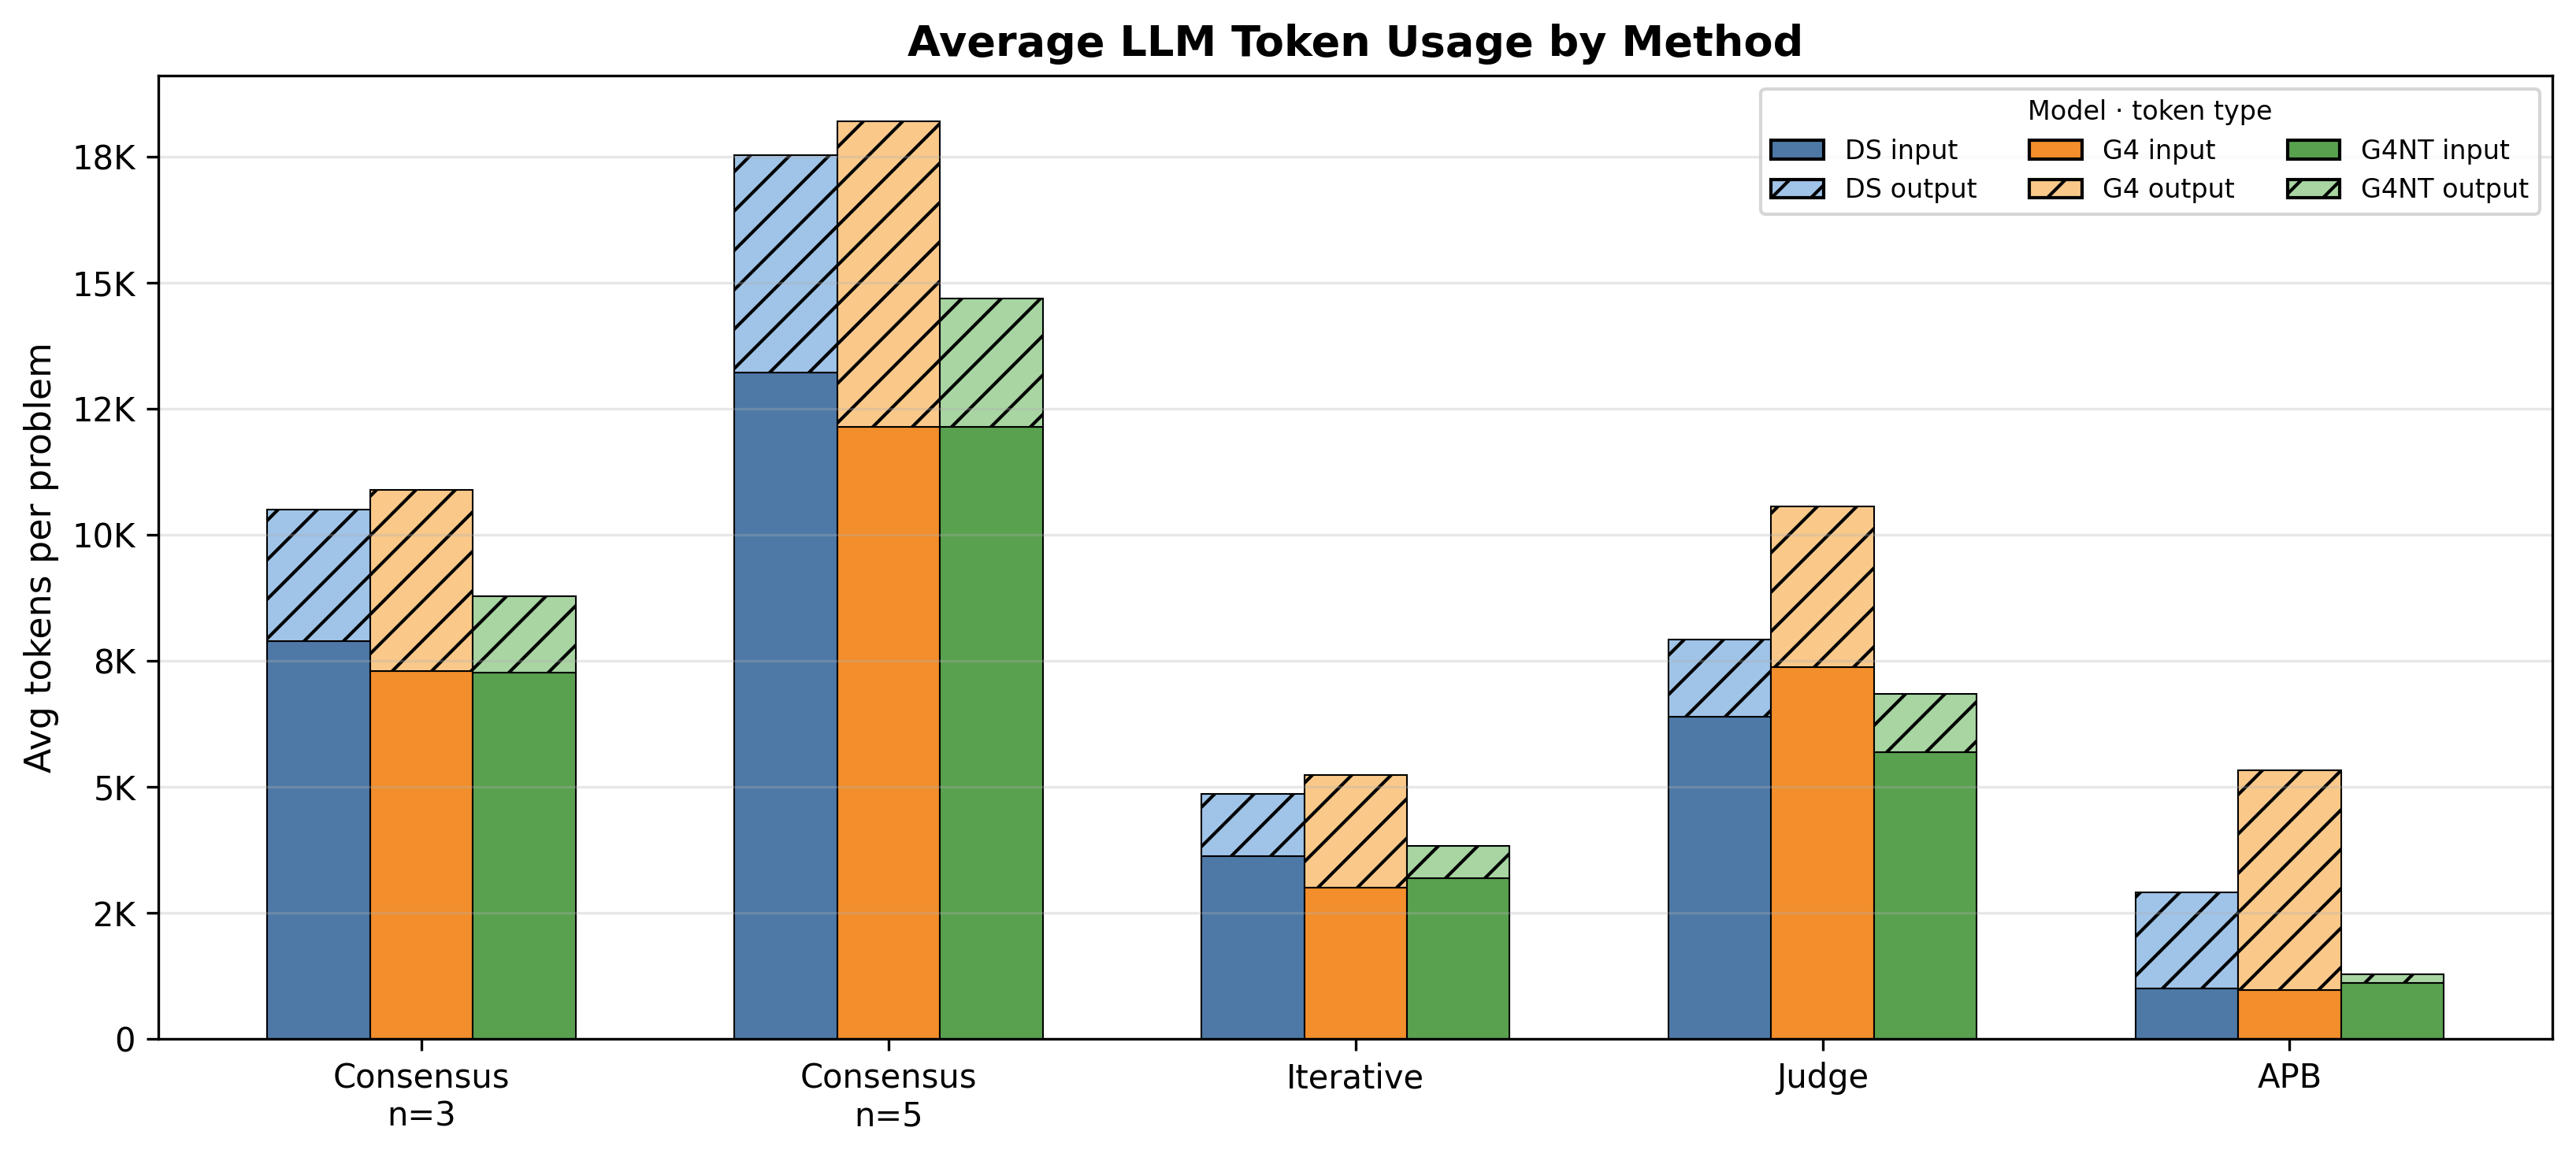
\includegraphics[width=0.45\textwidth]{figures/token_usage.png}
  \caption{\small{Average LLM token usage per problem (input: solid, output: hatched) across methods and models.}}
    \label{fig:token_usage}
\end{figure}

\subsubsection{Token Usage}
Figure~\ref{fig:token_usage} shows average LLM token usage per problem (input and output) across all domains and methods. The consensus methods incur the highest fixed cost, scaling directly with the number of samples: \textsc{n=5} consumes roughly twice the tokens of \textsc{n=3}, as each query is issued independently regardless of outcome. The judge approach falls between the two consensus variants --- it avoids the full \textsc{n=5} sample budget but pays an additional cost for the judge call and any subsequent re-queries when the judge is unsatisfied.

The iterative approach is the cheapest of the typing methods despite its looping behaviour. Unlike consensus, its lower bound is a single LLM query --- a valid plan after the first iteration requires no further calls --- which is reflected in the lower average cost. APB is cheapest overall, though its token profile is notably different: output tokens dominate for thinking-enabled models (\textsc{DS} and \textsc{G4}). \textsc{G4NT}, without a reasoning trace, has the lowest total cost across all methods.

\section{Discussion}

The results reveal no single dominant configuration, and instead each approach demonstrates distinct trade-offs between plan generation, refusal accuracy, and token cost. The iterative approach achieves the highest rate of successful plan generation on solvable problems and the lowest token cost, as its lower bound is a single LLM query. However, this comes at a cost: the looping structure prevents the system from refusing unsolvable problems under thinking-enabled models, which continue to search for a substitute even when none exists. Applications where false positives are dangerous should favor consensus or judge-based approaches, which preserve refusal accuracy with little sacrifice in plan generation performance.

Increasing the consensus sample count from $n{=}3$ to $n{=}5$ improves performance in some cases --- most notably on bulk problems where additional samples increase the chance of a correct majority vote --- but at roughly double the token cost. Whether this trade-off is worthwhile depends on the target domain; for problems where a single substitution is sufficient, $n{=}3$ is generally adequate.

Model selection has a meaningful impact beyond raw accuracy. Thinking-enabled models (\textsc{DS}, \textsc{G4}) are more willing to make creative type assignments, which benefits solvable problems but undermines refusal on unsolvable ones. \textsc{G4NT} presents a different profile: more conservative and literal, with comparable plan generation accuracy but substantially better refusal behaviour. This suggests that model choice should be informed by the application's tolerance for invalid substitutions. An interesting direction for future work would be a mixture-of-models consensus, combining the creative reasoning of thinking-enabled models with the conservatism of \textsc{G4NT} to improve both plan generation and refusal simultaneously.

\section{Real Robot Deployment}

The experiments above evaluate the typing step in isolation, on hand-authored problems. To show that this step composes into a working system rather than depending on curated PDDL, we deploy the full pipeline on a physical robot, where the typed problem is constructed end-to-end from raw perception rather than provided a priori.

Figure~\ref{fig:robot_example} shows the real robot domain, deployed on a Stretch mobile manipulator~\cite{stretch}. The domain includes actions such as \texttt{pickup} and \texttt{clean\_whiteboard}, each with typed preconditions that constrain which objects they can be applied to. At runtime, the scene is perceived using Grounding DINO~\cite{gdino} for open-vocabulary object detection and SAM 2~\cite{sam} for segmentation: the detector returns labeled bounding boxes for a set of prompted object classes, and SAM 2 refines these into pixel-level masks used to estimate each object's 3D position from aligned depth. The result is a set of detected objects with semantic class names --- the system knows, for example, that a \texttt{cloth} is present --- but has no knowledge of the affordances required by the planner. Accordingly, all detected objects are assigned the abstract base type \texttt{graspable} in the generated PDDL problem, and the LLM must assign appropriate types before planning can proceed. This is precisely the typing gap our method resolves, now arising organically from perception: the vision stack reports \emph{what} is in the scene, but not \emph{what role} each object can play.

The accompanying video shows the running example of Figure~\ref{fig:robot_example} executed on hardware: with no \texttt{eraser} present, the system types the \texttt{cloth} as a functional substitute and the robot completes the whiteboard-cleaning goal. We report the deployment as an integration demonstration rather than a quantitative benchmark by design. The claim under evaluation --- that the LLM resolves typing gaps correctly --- is measured in the controlled experiments above, where success depends only on the type assignment. Physical execution instead exercises orthogonal subsystems (grasping, navigation, depth estimation) whose failures are independent of typing correctness; folding them into a success metric would confound rather than test the contribution. The robot therefore establishes real-world applicability, while the benchmark establishes correctness.

\begin{figure}[t]
  \centering
  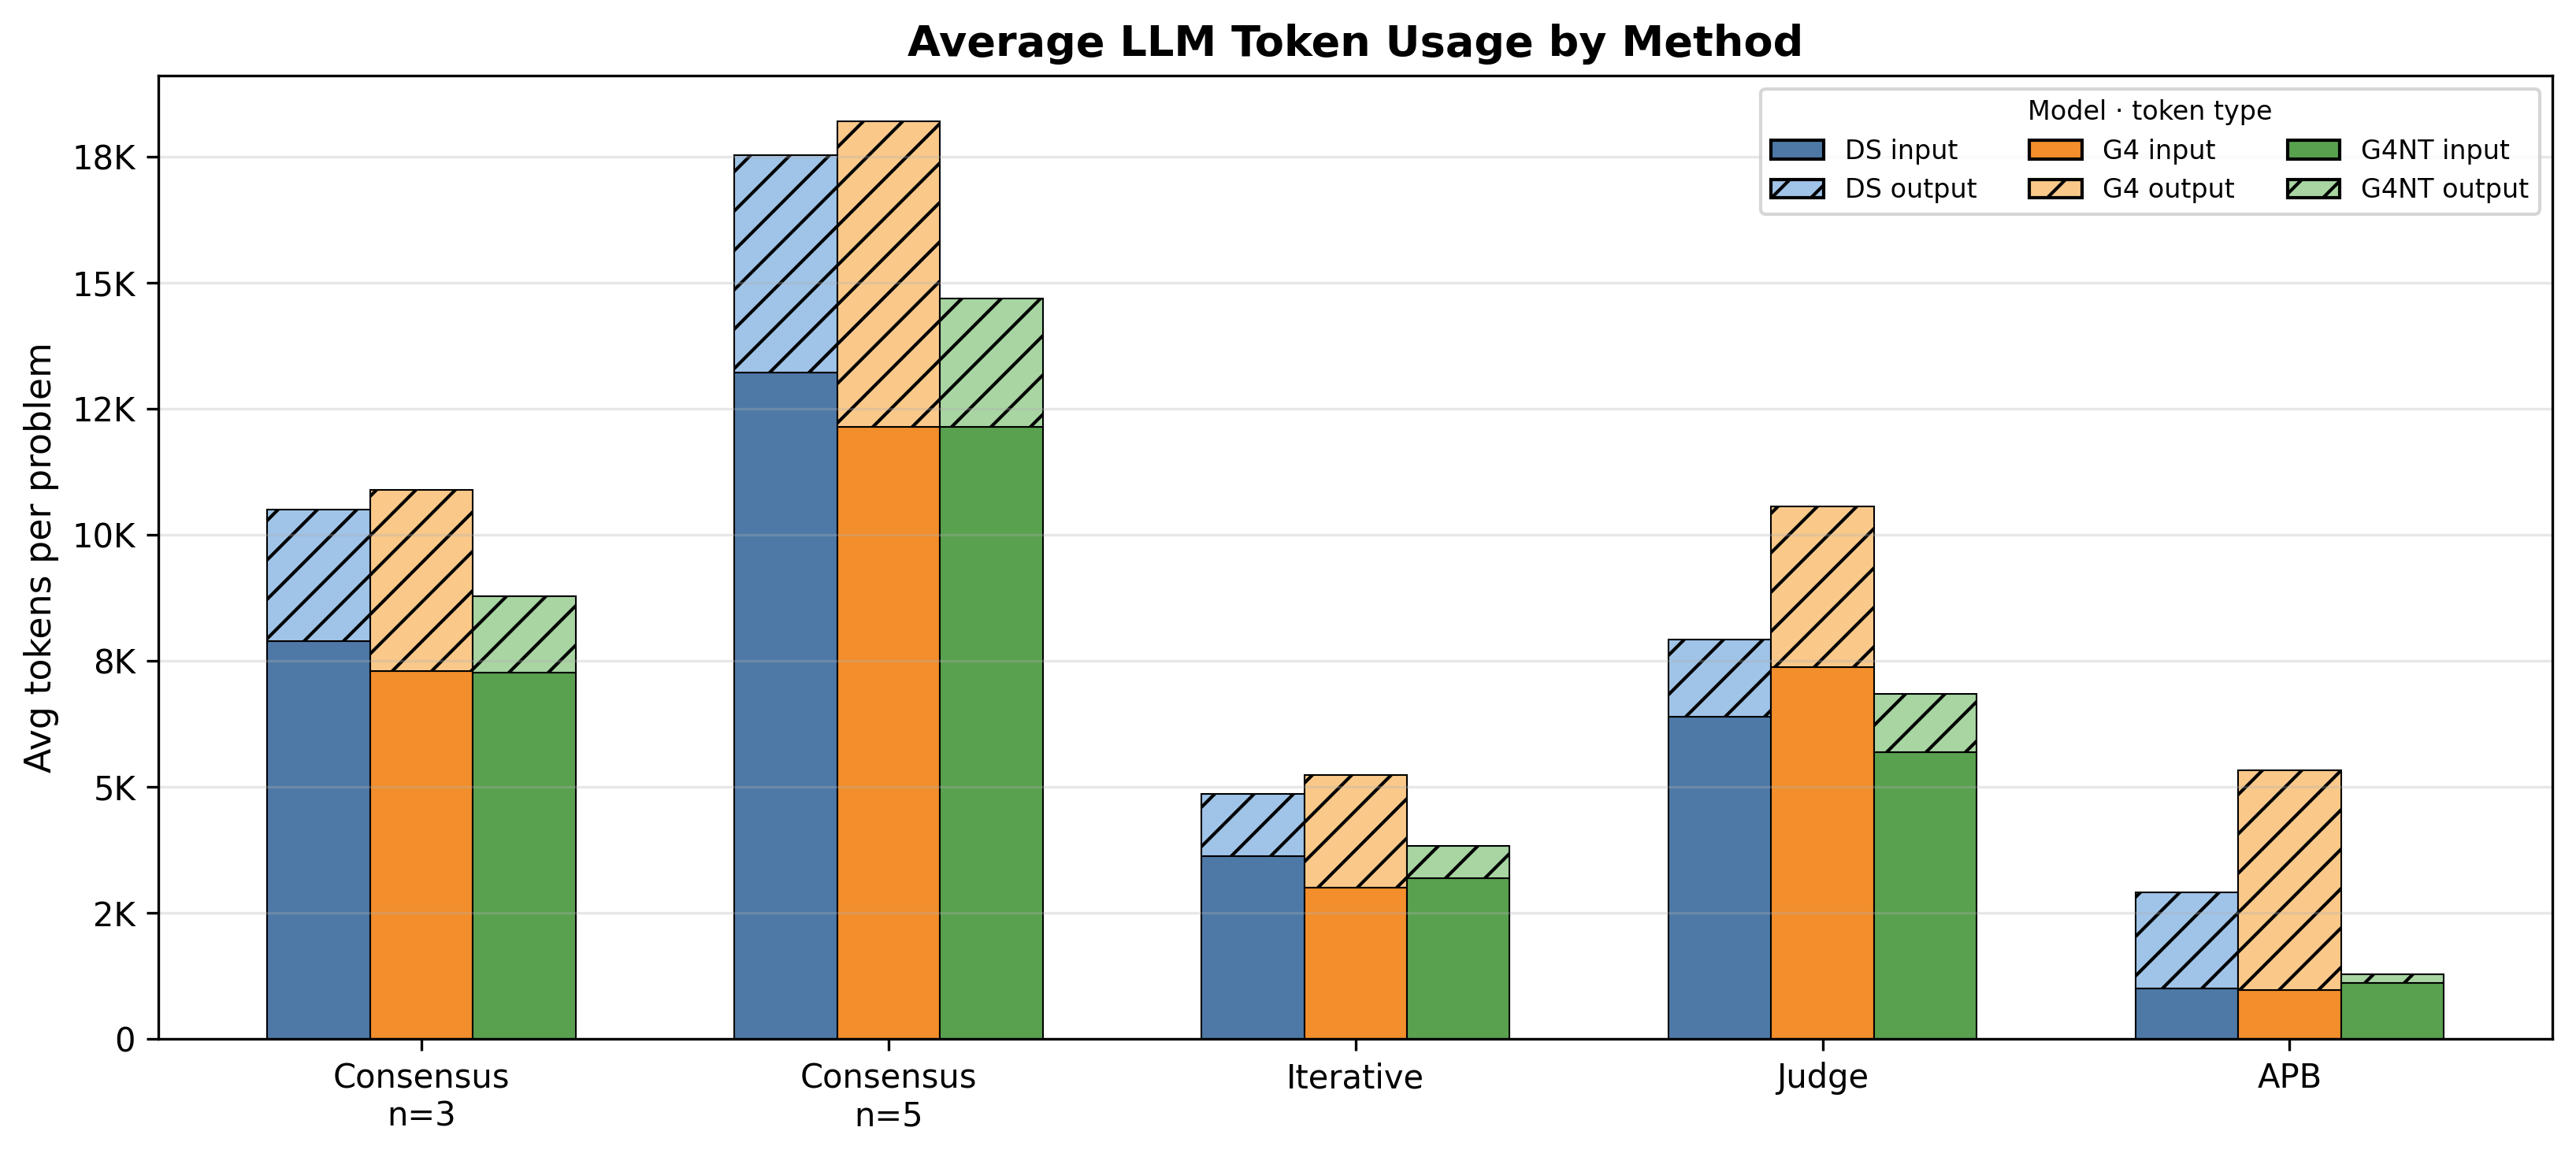
\includegraphics[width=0.45\textwidth]{figures/token_usage.png}
  \caption{\small{Average LLM token usage per problem (input: solid, output: hatched) across methods and models. Error bars show $\pm 1$ standard deviation of the total tokens per problem.}}
    \label{fig:token_usage}
\end{figure}

\section{Conclusion \& Future Work}

% We have shown that small, single-GPU open-weight LLMs, used across three CAST variants, can both recover valid plans for unsolvable problems and appropriately refuse when no valid substitution exists, substantially outperforming both LLM-based baselines across problem categories and semantic encodings. 

We introduced CAST, a neuro-symbolic component that operates upstream of a symbolic planner. CAST repairs runtime typing gaps by revising only the object-to-type assignments, making a minimal and constrained alteration to the symbolic knowledge used for planning.
Through our experiments, we show that CAST generally outperforms unconstrained PDDL repair and end-to-end LLM planning across substitution problems, distractor settings, and semantically varied domains. Our results also reveal a recovery--refusal trade-off: iterative refinement provides strong recovery at low token cost, whereas judge-based selection more reliably rejects invalid substitutions. A physical-robot demonstration further shows that CAST can be integrated into an open-vocabulary perception--planning--action pipeline.

Our approach has limitations that warrant further investigation. CAST offers no formal guarantees that substitutions made are valid. A \texttt{pick-up} action, for instance, may only apply to rigid objects and may not transfer to deformable ones. An avenue for future work can involve active probing for affordance discovery at runtime, enabling agents to test if actions can be successfully applied to an object before updating the symbolic representation. Additionally, we rely on the action name being semantically rich enough to describe its use; a less descriptive encoding like \texttt{action1} would give the LLM no signal about the affordances of \texttt{pickup-object} or which objects it applies to. Encoding affordances alongside actions, rather than relying on the action name alone, could give the LLM a more reliable signal for judging functional fit. 


\bibliography{references}

\appendix
\section{Consensus Sample-Count Ablation}
\label{app:consensus}

The main results report consensus at $n{=}3$. Here we ablate the number of samples
$n\in\{1,3,5\}$, where $n{=}1$ issues a single query with no voting or relaxation and
therefore isolates the model's single-shot accuracy. Table~\ref{tab:consensus_recovery}
reports recovery and Table~\ref{tab:consensus_refusal} refusal.

% ========== CONSENSUS RECOVERY ABLATION ==========
\begin{table*}[t]
\centering
\caption{Consensus recovery (\%) by sample count $n\in\{1,3,5\}$ (rows grouped by model). Recovery generally improves with $n$ but with diminishing returns, while token cost scales roughly linearly with $n$.}
\label{tab:consensus_recovery}
\footnotesize
\renewcommand{\arraystretch}{0.9}
\resizebox{\textwidth}{!}{%
\begin{tabular}{l|ccccc|cccc}
\toprule
 & \multicolumn{5}{c|}{\textbf{MacGyver Categories}} & \multicolumn{4}{c}{\textbf{Synonym Domains (single)}} \\
\midrule
\textbf{Config} & \textbf{single} & \textbf{bulk} & \textbf{stress-10} & \textbf{stress-20} & \textbf{stress-50} & \textbf{Electronics} & \textbf{Kitchen} & \textbf{Medic} & \textbf{Survival} \\
\midrule
DS-n1       & 86.0 $\pm$ 13.5 & 42.0 $\pm$ 39.4 & 78.0 $\pm$ 31.9 & 86.0 $\pm$ 21.2 & 56.0 $\pm$ 29.5 & 86.0 $\pm$ 13.5 & 70.0 $\pm$ 28.7 & 98.0 $\pm$ 6.3 & 90.0 $\pm$ 17.0 \\
DS-n3       & \textbf{100.0} $\pm$ 0.0 & 54.0 $\pm$ 38.9 & 86.0 $\pm$ 29.9 & 82.0 $\pm$ 29.0 & 88.0 $\pm$ 21.5 & 98.0 $\pm$ 6.3 & 88.0 $\pm$ 16.9 & \textbf{100.0} $\pm$ 0.0 & 96.0 $\pm$ 12.6 \\
DS-n5       & \textbf{100.0} $\pm$ 0.0 & 58.0 $\pm$ 50.3 & 90.0 $\pm$ 25.4 & 82.0 $\pm$ 29.0 & 86.0 $\pm$ 21.2 & \textbf{100.0} $\pm$ 0.0 & 92.0 $\pm$ 14.0 & 98.0 $\pm$ 6.3 & \textbf{100.0} $\pm$ 0.0 \\
\midrule
G4-n1       & \textbf{100.0} $\pm$ 0.0 & 60.0 $\pm$ 51.6 & \textbf{100.0} $\pm$ 0.0 & \textbf{100.0} $\pm$ 0.0 & \textbf{100.0} $\pm$ 0.0 & \textbf{100.0} $\pm$ 0.0 & 98.0 $\pm$ 6.3 & \textbf{100.0} $\pm$ 0.0 & 98.0 $\pm$ 6.3 \\
G4-n3       & \textbf{100.0} $\pm$ 0.0 & 60.0 $\pm$ 51.6 & \textbf{100.0} $\pm$ 0.0 & \textbf{100.0} $\pm$ 0.0 & \textbf{100.0} $\pm$ 0.0 & \textbf{100.0} $\pm$ 0.0 & \textbf{100.0} $\pm$ 0.0 & \textbf{100.0} $\pm$ 0.0 & 98.0 $\pm$ 6.3 \\
G4-n5       & \textbf{100.0} $\pm$ 0.0 & 60.0 $\pm$ 51.6 & \textbf{100.0} $\pm$ 0.0 & \textbf{100.0} $\pm$ 0.0 & \textbf{100.0} $\pm$ 0.0 & \textbf{100.0} $\pm$ 0.0 & \textbf{100.0} $\pm$ 0.0 & \textbf{100.0} $\pm$ 0.0 & \textbf{100.0} $\pm$ 0.0 \\
\midrule
G4NT-n1     & \textbf{100.0} $\pm$ 0.0 & \textbf{64.0} $\pm$ 39.8 & \textbf{100.0} $\pm$ 0.0 & \textbf{100.0} $\pm$ 0.0 & 98.0 $\pm$ 6.3 & \textbf{100.0} $\pm$ 0.0 & 98.0 $\pm$ 6.3 & \textbf{100.0} $\pm$ 0.0 & \textbf{100.0} $\pm$ 0.0 \\
G4NT-n3     & \textbf{100.0} $\pm$ 0.0 & 58.0 $\pm$ 50.3 & \textbf{100.0} $\pm$ 0.0 & \textbf{100.0} $\pm$ 0.0 & \textbf{100.0} $\pm$ 0.0 & \textbf{100.0} $\pm$ 0.0 & \textbf{100.0} $\pm$ 0.0 & \textbf{100.0} $\pm$ 0.0 & \textbf{100.0} $\pm$ 0.0 \\
G4NT-n5     & \textbf{100.0} $\pm$ 0.0 & \textbf{64.0} $\pm$ 47.9 & \textbf{100.0} $\pm$ 0.0 & \textbf{100.0} $\pm$ 0.0 & \textbf{100.0} $\pm$ 0.0 & \textbf{100.0} $\pm$ 0.0 & \textbf{100.0} $\pm$ 0.0 & \textbf{100.0} $\pm$ 0.0 & \textbf{100.0} $\pm$ 0.0 \\
\bottomrule
\end{tabular}}
\end{table*}

\paragraph{Recovery.} Recovery generally improves with $n$ but with diminishing returns:
on \textsc{single} and \textsc{stress} the Gemma4 variants are already saturated at
$n{=}1$, and the largest gains appear on \textsc{bulk} and for \textsc{Deepseek}, whose
single-shot accuracy is lower. Because token cost scales roughly linearly with $n$
(about $3.7$k, $11$k, and $18$k tokens per problem at $n{=}1,3,5$), $n{=}3$ is a
reasonable default and $n{=}5$ rarely justifies its cost.

% ========== CONSENSUS REFUSAL ABLATION ==========
\begin{table}[t]
\centering
\caption{Consensus refusal accuracy on \textsc{no\_sub} problems by sample count. Refusal \emph{degrades} as $n$ grows: vote-rank relaxation searches harder for a solvable assignment and, on an unsolvable problem, is more likely to accept a distractor. \textsc{Deepseek} collapses at $n{=}5$.}
\label{tab:consensus_refusal}
\footnotesize
\renewcommand{\arraystretch}{0.9}
\resizebox{\columnwidth}{!}{%
\begin{tabular}{l|ccc|c}
\toprule
\textbf{Method} & \textbf{DS} & \textbf{G4} & \textbf{G4NT} & \textbf{Avg} \\
\midrule
Cons n=1   & \textbf{64.0} $\pm$ 36.3 & \textbf{66.0} $\pm$ 47.2 & \textbf{52.0} $\pm$ 48.3 & \textbf{60.7} $\pm$ 7.6 \\
Cons n=3   & 60.0 $\pm$ 32.7 & 56.0 $\pm$ 46.0 & 50.0 $\pm$ 46.4 & 55.3 $\pm$ 5.0 \\
Cons n=5   & 16.0 $\pm$ 18.4 & 62.0 $\pm$ 44.7 & 48.0 $\pm$ 48.3 & 42.0 $\pm$ 23.6 \\
\bottomrule
\end{tabular}}
\end{table}

\paragraph{Refusal.} Refusal moves in the opposite direction --- it \emph{degrades} as
$n$ grows. This is a direct consequence of the consensus vote-rank relaxation, which on
planner failure re-types low-confidence objects to any alternative that received a vote,
searching for a solvable assignment. On an unsolvable problem this search is exactly what
should be avoided, and it worsens with the sample budget: more samples accumulate more
distractor$\rightarrow$tool proposals, so relaxation is more likely to find one the
planner accepts. \textsc{Deepseek} at $n{=}5$ is the extreme case, collapsing to $16\%$
from $64\%$ and $60\%$ at $n{=}1$ and $n{=}3$; of its $42$ false positives, $28$ were
produced by relaxation retyping a distractor such as \texttt{ripe-banana} to
\texttt{hammer}. The mechanism that aids recovery thus directly undermines refusal, which
is why the main results adopt the more conservative $n{=}3$.


\end{document}
